\documentclass[11pt,a4paper]{article}

% ---------------------------------------------------------------------------
% Conservative exchange preserves repeated production in autocatalytic
% reactor networks: a uniform composition theorem with a machine-checked proof.
%
% Author metadata: set the macros below before submission.  They are
% deliberately left blank in this version.  \CompanionAuthor is the author
% printed for the companion manuscripts in refs.bib; \RepositoryNote is where
% the public repository location goes.
% ---------------------------------------------------------------------------
\newcommand{\PaperAuthor}{}
\newcommand{\PaperAffiliation}{}
\newcommand{\PaperDate}{16 September 2026}
\newcommand{\CompanionAuthor}{Anonymous}
\newcommand{\RepositoryNote}{The repository location will be supplied with the author information.}

\usepackage[T1]{fontenc}
\usepackage[utf8]{inputenc}
\usepackage{lmodern}
\usepackage{microtype}
\usepackage[a4paper,margin=1.05in]{geometry}
\usepackage{amsmath,amssymb,amsthm,mathtools}
\usepackage{booktabs}
\usepackage{array}
\usepackage{longtable}
\usepackage{enumitem}
\usepackage{xcolor}
\usepackage{graphicx}
\usepackage{tikz}
\usetikzlibrary{arrows.meta,positioning,calc}
\usepackage[obeyspaces,spaces]{url}
\usepackage[numbers,sort&compress]{natbib}
\usepackage[colorlinks=true,linkcolor=blue!55!black,citecolor=blue!55!black,urlcolor=blue!55!black]{hyperref}
\hypersetup{pdftitle={Conservative exchange preserves repeated production in autocatalytic reactor networks},
  pdfkeywords={autocatalysis, reactor networks, composition, comparison principle, impulsive differential equations, chemical reaction networks, Lean}}

\DeclareUrlCommand\lean{\urlstyle{tt}}
\setlist{itemsep=2pt,topsep=3pt}
\setlength{\emergencystretch}{1.5em}
\graphicspath{{figures/}}

\theoremstyle{plain}
\newtheorem{theorem}{Theorem}[section]
\newtheorem{proposition}[theorem]{Proposition}
\newtheorem{lemma}[theorem]{Lemma}
\newtheorem{corollary}[theorem]{Corollary}
\theoremstyle{definition}
\newtheorem{definition}[theorem]{Definition}
\theoremstyle{remark}
\newtheorem{remark}[theorem]{Remark}

\newcommand{\R}{\mathbb R}
\newcommand{\eps}{\varepsilon}
\newcommand{\dd}{\,\mathrm d}
\newcommand{\Adm}{\mathcal C}
\newcommand{\Bstar}{\mathcal B_*}
\newcommand{\Pulse}{\Pi}
\newcommand{\Iv}{I}
\newcommand{\Dop}{D}
\newcommand{\Pnet}{P_{\mathrm{net}}}
\newcommand{\umol}{\,\mu\mathrm{mol}}
\newcommand{\nmol}{\,\mathrm{nmol}}

\title{Conservative exchange preserves repeated production\\ in autocatalytic reactor networks:\\[4pt]
\large a uniform composition theorem with a machine-checked proof}
\author{\PaperAuthor\\ \small \PaperAffiliation}
\date{\PaperDate}

\begin{document}
\maketitle

\begin{abstract}
An isolated reactor's guarantee of repeated productive operation does not automatically survive connection to other reactors: exchange changes the state during recovery, and the exchanged material includes the catalyst in all of its chemical forms. We prove that it does survive for a specified family. Any finite number of equal-volume, maintained, reversible six-species autocatalytic reactors, each with its own release and cleavage speeds in a fixed rectangle, is connected by an arbitrary finite symmetric nonnegative exchange graph in which every edge transports all six internal species with one common coefficient. Synchronized harvesting interventions withdraw a quarter to three quarters of each reactor, allow up to two percent additional species-dependent loss, refill only food with a bounded error, and may depend on the completed history of the whole assembly. From any admitted preparation, one pulse and twelve normalized time units carry the assembly into an operating region; thereafter every pulse followed by four units of flow returns the actual coupled state to that region, and the last unit of every cycle collects at every node at least $1/28$ template equivalents and at least $1/160$ of the free template species, with explicit food and driven-service allowances that are linear in the number of cycles. The constants do not depend on the number of reactors, the graph, or the exchange strength. The proof rests on three properties of common transport (it commutes with fixed linear observables, is nonnegative at a node that minimizes such an observable, and cancels from summed accounts), a finite simultaneous comparison principle that never differentiates a moving minimum, guarded catalytic growth at the least-stock node, and a backward-evolving phase observable that converts complexed stock into a free-product guarantee; a degree-four truncation of the backward weight improves an earlier floor of $1/209$ to $1/160$. An inventory telescope proves net synthesis beyond the initial template stock. An exact two-node witness shows that species-selective exchange breaks the minimum-drift argument. The trajectory, return, output, resource, arbitrary-repetition and net-synthesis statements are verified in Lean~4 as one declaration, together with closed path and ring instances; conventional corollaries give mission sizing, endpoint rates and architecture-dependent handling bounds, and a dimensioned four-reactor array with numerical diagnostics illustrates the constants without asserting a molecular realization.
\end{abstract}

\section{Introduction}\label{sec:intro}

The structural theory of autocatalysis, from autocatalytic sets~\citep{kauffman1986} and the RAF formalism~\citep{hordijk2004,steel2019} to the stoichiometric classification of autocatalytic cores~\citep{blokhuis2020}, certifies that a network can regenerate its catalysts from food. Whether a particular maintained reactor can be harvested repeatedly is a dynamical question in the tradition of serial-transfer experiments~\citep{mills1967,lincoln2009,vaidya2012}: after each withdrawal the disturbed state must regrow, through its own kinetics, into a state from which the next withdrawal is admissible. A companion paper~\citep{recovery2026} proves such a repeated-harvesting theorem, with explicit constants and a machine-checked proof, for the deterministic mass-action dynamics of a thermochemically consistent six-species autocatalytic exporter~\citep{thermo2026}.

Reactors are rarely operated alone. Designed enzymatic and organic reaction networks are run in linked flow modules whose function depends on the connection as much as on the chemistry~\citep{semenov2015,semenov2016}, and open reaction networks compose along shared boundary species~\citep{baez2017}. This raises a preservation question that structural theory does not answer: \emph{which operating guarantees of a module survive a declared connection rule?} Connection is not harmless. Exchange moves the catalyst between reactors in every one of its chemical forms while each reactor is still recovering; it can lower the stock of a reactor that was about to be harvested; and it makes the return condition at the next intervention a statement about the whole coupled nonlinear state, not about one reactor at a time. A composition theorem must follow the coupled trajectory, prove that its actual endpoint admits the next intervention at every node, and count output and expenditure along that same history.

This paper proves such a theorem for the family obtained by connecting any finite number of the reactors of~\citep{recovery2026} through \emph{conservative nonselective exchange}: a symmetric nonnegative graph on the reactors, with every internal species transported along an edge at the same coefficient. Node kinetics may differ within the rectangle of the isolated theorem, interventions are synchronized but may differ by node and depend on the completed history of the assembly, and no bound on the exchange strength, no connectedness, and no equilibrium or linearization is assumed. The transport operator is the weighted graph Laplacian of compartmental exchange~\citep{jacquez1993}, and the proof uses exactly three of its properties: it commutes with every fixed linear combination of species, it is nonnegative at a node where such a combination is smallest, and it cancels from the sum over nodes when the graph is symmetric. The first two preserve every recovery estimate of the isolated reactor without any penalty proportional to the exchange strength; the third prevents internal transfers from being counted as output or fresh supply.

\paragraph{Contributions.}
\begin{enumerate}[label=(\roman*)]
\item \emph{A uniform composition theorem} (Theorem~\ref{thm:main}). From any admitted assembly, one pulse and twelve time units reach the operating region $\Bstar^N$; from $\Bstar^N$ every synchronized admissible pulse, followed by four units of coupled flow, returns the actual endpoint to $\Bstar^N$, with catalytic stock recovered by time $5/2$ and full readiness from time $3$; the fourth unit collects at every node at least $1/28$ template equivalents and at least $1/160$ free template. The constants are independent of the number of nodes, the graph and the exchange coefficients, and the theorem constructs the coupled trajectories rather than assuming them.
\item \emph{Mechanism.} A finite simultaneous comparison principle (Lemma~\ref{lem:comparison}) propagates a common lower bound through the graph without differentiating a changing minimum. The elemental totals of every node contract to their fixed point at unit rate under any exchange (Lemma~\ref{lem:material}). Guarded catalytic growth holds at the node of least weighted stock because transport is nonnegative there (Lemma~\ref{lem:growth}), so the strict exponential fence of the isolated theorem carries over with the same deadlines (Lemma~\ref{lem:fence}).
\item \emph{Free product through a backward observable} (Section~\ref{sec:phase}). Complexed catalyst is not harvestable free product. A row vector of phase weights that evolves backward from the observation time cancels the favourable phase-transfer terms of a positive lower comparison system, and the same comparison principle propagates its minimum through the network (Lemma~\ref{lem:backward}). Two explicit certificates result: a nilpotent one giving the floor $1/209$, and a degree-four truncation retaining the distinct phase losses and the duplex-to-complex link, giving $1/160$ (Proposition~\ref{prop:floor}). Both improve the first compiled floor $1/540$.
\item \emph{Accounts and net synthesis.} Transport cancels from the summed template inventory, so an integrated inventory identity telescoped over cycles proves net synthesis beyond the initial stock: positive from the twenty-ninth routine cycle from a ready start and from the thirty-first after conditioning (Proposition~\ref{prop:synthesis}). Food, driven-service and gross-handling accounts are explicit; the handling allowance is the only architecture-dependent cost (Section~\ref{sec:consequences}).
\item \emph{Boundary of the connection rule.} An exact rational two-node witness shows that species-selective exchange (free template only) makes the drift of the weighted stock negative at a node of minimal stock, so the minimum-drift argument does not extend to selective transport (Proposition~\ref{prop:selective}).
\item \emph{Verification and diagnostics.} The trajectory, return, output, resource, arbitrary-repetition and net-synthesis statements are verified in Lean~4~\citep{demoura2021} with Mathlib~\citep{mathlib2020} as one declaration, together with closed four-node path and ring instances (Appendix~\ref{app:formal}). A dimensioned four-reactor array and a four-run numerical pilot measure how conservative the constants are (Section~\ref{sec:units}); an exact replay script re-derives every printed number.
\end{enumerate}

\paragraph{Relation to existing tools.}
Invariant regions and comparison functions for reaction--diffusion systems are classical~\citep{chueh1977,walter1970}, cooperative systems preserve order~\citep{hirsch2005}, and compartmental transport is well understood~\citep{jacquez1993}. We claim no novelty for the maximum principle itself; the finite-graph argument is given in full because the formal proof follows it. The contribution is the explicit transient preservation implication for this source: disturbed coupled states recover, return, and support repeated collection with uniform quantitative bounds, all from one local growth inequality and one phase observable. Open-network thermodynamics~\citep{polettini2014,rao2016} supplies the distinction between the gross driven service counted here and the total work of an apparatus.

\paragraph{Three kinds of evidence.}
Three kinds of statement appear and are kept apart. The source identities, the existence and uniqueness of nonnegative coupled trajectories, the finite comparison principle, material contraction, guarded growth, the fence, both phase certificates, the output, food and service integrals, arbitrary history-dependent repetition, the inventory telescope and net synthesis are Lean-verified; Appendix~\ref{app:formal} maps each claim to a declaration. Mission sizing, endpoint rates, handling and material ceilings, dimensional conversions, the dilution derivation and the unequal-volume remark are conventional arguments written out in full and labelled as such. The numerical pilot is a diagnostic and proves nothing.

\paragraph{What is not claimed.}
The model is schematic chemistry with three formal elemental components, maintained fuel and waste activities, ideal mass action, one effective trimolecular reverse channel, equal reactor volumes, instantaneous synchronized pulses and bulk nonselective exchange. No laboratory molecule is identified and no rate is fitted. Handling and driven-service counters measure specified parts of reactor operation, not pumping energy or total apparatus work. No equilibrium convergence, synchronization, periodic-orbit attraction, stochastic reliability, asynchronous operation, membrane selectivity or autonomous finite-bath dynamics is asserted; Section~\ref{sec:scope} states exactly what each of these would require.

\paragraph{Organization.}
Section~\ref{sec:model} specifies the coupled source, the interventions and the state regions. Section~\ref{sec:main} states the theorem. Sections~\ref{sec:transport}--\ref{sec:repetition} prove it: transport and comparison (Section~\ref{sec:transport}), material and catalytic recovery (Section~\ref{sec:recovery}), free product (Section~\ref{sec:phase}), repetition, accounts and net synthesis (Section~\ref{sec:repetition}). Section~\ref{sec:consequences} derives operational consequences, Section~\ref{sec:units} a dimensioned array with diagnostics, Section~\ref{sec:scope} the transport boundary and scope, and Section~\ref{sec:discussion} the discussion. Appendix~\ref{app:formal} contains the formal evidence and reproduction commands.

\section{The coupled source and the operating protocol}\label{sec:model}

\subsection{Local chemistry and the coupled field}\label{sec:chemistry}
There are $N\ge1$ well-mixed reactors of equal constant volume, indexed by $i$. The internal species are two foods $U,W$, the free template $X$, two complexes $C_1,C_2$ and a duplex $Z$; a fuel $F$ and a waste $P$ are maintained at unit activity. The state of node $i$ is
\[
c_i=(u_i,w_i,x_i,c_{1i},c_{2i},z_i)\in\R^6_{\ge0},
\]
with concentrations and time normalized until Section~\ref{sec:units}. Put
\begin{equation}\label{eq:parameters}
\eps=\frac1{500\,000\,000},\qquad \eta=\frac1{8\,000\,000\,000},\qquad
19\le r_i\le21,\qquad \frac1{50}\le\delta_i\le\frac1{25},
\end{equation}
where the release speed $r_i$ and the cleavage speed $\delta_i$ of node $i$ are fixed throughout an operation and may differ between nodes. The six reversible pairs and their net forward fluxes at node $i$ are those of~\citep{recovery2026}, listed in Table~\ref{tab:pairs}. Pairs $1$--$4$ form the templated path $X+U+W\to C_1\to C_2\to Z\to2X$, which is the autocatalytic completion; pair $0$ is basal formation; pair $5$ is driven cleavage by the fuel, whose reverse is an effective trimolecular step. Each food enters at unit rate and every internal species washes out at unit rate, so the local field is
\begin{equation}\label{eq:field}
f_{r,\delta}(c)=\begin{pmatrix}
1-u-j_0-j_1+j_5\\1-w-j_0-j_2+j_5\\-x+j_0-j_1+2j_4-j_5\\
-c_1+j_1-j_2\\-c_2+j_2-j_3\\-z+j_3-j_4
\end{pmatrix}.
\end{equation}

\begin{table}[tb]
\centering\small
\begin{tabular}{clll}
\toprule
Index & Reversible pair & Net forward flux & Role\\
\midrule
0 & $U+W\rightleftharpoons X$ & $j_0=\eps\,uw-(\eps/10)\,x$ & basal formation\\
1 & $X+U\rightleftharpoons C_1$ & $j_1=20\,xu-20\,c_1$ & substrate binding\\
2 & $C_1+W\rightleftharpoons C_2$ & $j_2=20\,c_1w-20\,c_2$ & substrate binding\\
3 & $C_2\rightleftharpoons Z$ & $j_3=20\,c_2-2\,z$ & templated ligation\\
4 & $Z\rightleftharpoons 2X$ & $j_4=r\,(z-x^2)$ & duplex release\\
5 & $X+F\rightleftharpoons U+W+P$ & $j_5=\delta\,x-\delta\eta\,uw$ & driven cleavage\\
\bottomrule
\end{tabular}
\caption{The six reversible pairs at unit fuel and waste activities; $r$ and $\delta$ scale both directions of their pairs.}
\label{tab:pairs}
\end{table}

Fix exchange coefficients $k_{ij}=k_{ji}\ge0$ with $k_{ii}=0$; no connectedness and no upper bound is imposed. The exchange operator and the coupled field are
\begin{equation}\label{eq:source}
(\Dop v)_i=\sum_{j}k_{ij}(v_j-v_i),\qquad
\dot c_{is}=f_{r_i,\delta_i}(c_i)_s+(\Dop c_{\cdot s})_i\quad(s=1,\dots,6).
\end{equation}
The same operator acts on all six species: exchange is \emph{nonselective}. At the level of events, the location-labelled transfer of one unit of species $s$ from node $i$ to node $j$ has rate $k_{ij}c_{is}$ and increment $-e_{is}+e_{js}$; summing all such directed transfers gives exactly the transport term in~\eqref{eq:source}. Every transfer has zero external-food and zero product-export marks and one gross-handling mark, so an undirected edge carries twelve directed species labels. Figure~\ref{fig:network} shows the module and three admissible graphs.

\begin{figure}[tb]
\centering
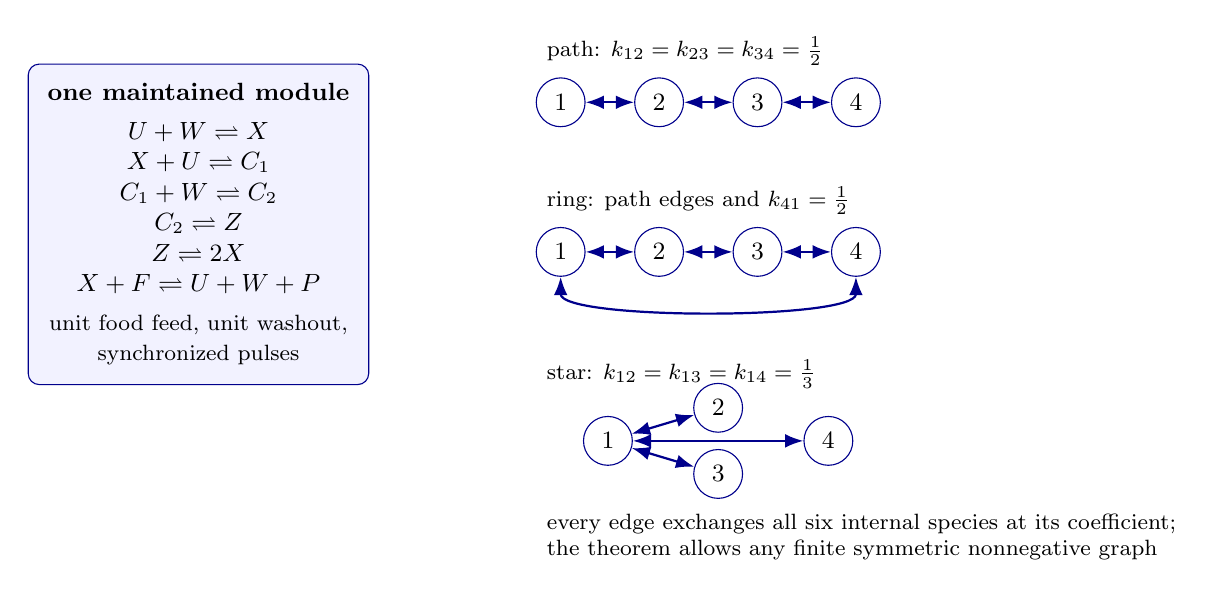
\begin{tikzpicture}[>=Latex,
  nd/.style={circle,draw=blue!55!black,fill=white,minimum size=0.62cm,inner sep=0pt,font=\small},
  ed/.style={<->,thick,blue!55!black},
  lab/.style={font=\footnotesize}]
\node[draw=blue!55!black,fill=blue!5,rounded corners=4pt,inner sep=7pt,align=center,font=\small] (mod) at (0,0)
 {\textbf{one maintained module}\\[3pt]
  $U+W\rightleftharpoons X$\\ $X+U\rightleftharpoons C_1$\\ $C_1+W\rightleftharpoons C_2$\\ $C_2\rightleftharpoons Z$\\ $Z\rightleftharpoons 2X$\\ $X+F\rightleftharpoons U+W+P$\\[3pt]
  \footnotesize unit food feed, unit washout,\\ \footnotesize synchronized pulses};
\begin{scope}[shift={(4.6,1.55)}]
 \node[lab,anchor=west] at (-0.3,0.65) {path: $k_{12}=k_{23}=k_{34}=\tfrac12$};
 \foreach \i in {1,2,3,4} \node[nd] (p\i) at ({1.25*(\i-1)},0) {\i};
 \draw[ed] (p1)--(p2); \draw[ed] (p2)--(p3); \draw[ed] (p3)--(p4);
\end{scope}
\begin{scope}[shift={(4.6,-0.35)}]
 \node[lab,anchor=west] at (-0.3,0.65) {ring: path edges and $k_{41}=\tfrac12$};
 \foreach \i in {1,2,3,4} \node[nd] (r\i) at ({1.25*(\i-1)},0) {\i};
 \draw[ed] (r1)--(r2); \draw[ed] (r2)--(r3); \draw[ed] (r3)--(r4);
 \draw[ed] (r4.south) .. controls ($(r4.south)+(0,-0.55)$) and ($(r1.south)+(0,-0.55)$) .. (r1.south);
\end{scope}
\begin{scope}[shift={(4.6,-2.75)}]
 \node[lab,anchor=west] at (-0.3,0.85) {star: $k_{12}=k_{13}=k_{14}=\tfrac13$};
 \node[nd] (s1) at (0.6,0) {1};
 \node[nd] (s2) at (2.0,0.42) {2}; \node[nd] (s3) at (2.0,-0.42) {3}; \node[nd] (s4) at (3.4,0) {4};
 \draw[ed] (s1)--(s2); \draw[ed] (s1)--(s3); \draw[ed] (s1)--(s4);
\end{scope}
\node[lab,align=left,anchor=north west] at (4.3,-3.55) {every edge exchanges all six internal species at its coefficient;\\ the theorem allows any finite symmetric nonnegative graph};
\end{tikzpicture}
\caption{The local module and the three four-node exchange graphs used in Sections~\ref{sec:units} and~\ref{app:formal}. Double arrows denote bidirectional internal exchange, not external collection. Food input and washout act at every node.}
\label{fig:network}
\end{figure}

\subsection{Elemental balance and common thermochemistry}\label{sec:thermo}
Assign three formal elemental units $U=(1,0,0)$, $W=(0,1,0)$, $X=(1,1,0)$, $C_1=(2,1,0)$, $C_2=Z=(2,2,0)$, $F=P=(0,0,1)$. Every pair balances each unit. In units of thermal energy the standard potentials
\begin{equation}\label{eq:potential}
\mu^\circ=\bigl(0,\,0,\,-\log10,\,-\log10,\,-\log10,\,-2\log10,\,\log(8\cdot10^{10}),\,0\bigr)
\end{equation}
in the order $U,W,X,C_1,C_2,Z,F,P$ satisfy $\log(k_j^+/k_j^-)=$ reactant minus product potential sum for every pair and every $(r,\delta)$, because $r$ and $\delta$ scale both directions. A transfer event relocates a molecule without changing any location-independent property, so it balances every elemental unit and every potential; with identical potentials at all nodes the symmetric transfer coefficients are compatible with the same assignment. This establishes algebraic consistency of the model~\citep{thermo2026}, not the existence of molecules with these properties.

\subsection{Interventions and policies}\label{sec:pulse}
\begin{definition}[Admissible intervention]\label{def:pulse}
An intervention is $p=(q,\ell,e_U,e_W)$ with
\begin{equation}\label{eq:pulsebounds}
\tfrac14\le q\le\tfrac34,\qquad \tfrac{49}{50}\le\ell_s\le1\ \ (s=1,\dots,6),\qquad |e_U|,\ |e_W|\le\tfrac1{200}.
\end{equation}
Its pulse map retains $q\ell_sc_s$ of every species and adds food:
\begin{equation}\label{eq:pulse}
(\Pulse_pc)_s=q\ell_sc_s+\mathbf 1_{s=U}(1-q+e_U)+\mathbf 1_{s=W}(1-q+e_W).
\end{equation}
The withdrawn state is $(1-q)c$, the additionally lost state is $q(1-\ell)c$, and retained, withdrawn and lost states sum to $c$. Refill adds no catalyst-bearing species.
\end{definition}
A synchronized intervention on the assembly is a vector $p=(p_1,\dots,p_N)$ of admissible interventions applied simultaneously, one per node; write $\Pulse_pc=(\Pulse_{p_1}c_1,\dots,\Pulse_{p_N}c_N)$. A \emph{policy} is any function $\Pi$ that assigns to the cycle index $n$, the list of completed earlier routine segments and the current assembly state a synchronized intervention. No regularity is required: each pulse occurs at a discrete time, sees only completed data, and produces admissible data for the next flow segment. The pulse has zero modelled duration and the volume is restored externally; Section~\ref{sec:dilution} shows that~\eqref{eq:pulse} is the endpoint map of a withdrawal followed by a volume-restoring refill.

\subsection{Observables, regions and credited output}\label{sec:regions}
Four linear observables organize the analysis:
\begin{equation}\label{eq:observables}
\begin{aligned}
A&=u+x+2c_1+2c_2+2z,&B&=w+x+c_1+2c_2+2z,\\
Y&=x+\tfrac98c_1+\tfrac75c_2+\tfrac95z,&\Iv&=x+c_1+c_2+2z.
\end{aligned}
\end{equation}
$A$ and $B$ count the two food elemental units among internal species, $Y$ is a weighted catalytic stock used as a proof device, and $\Iv$ counts template equivalents across all phases (two for the duplex). For a nonnegative state $\Iv\le A$, $\Iv\le B$ and
\begin{equation}\label{eq:IY}
\Iv-\tfrac57Y=\tfrac27x+\tfrac{11}{56}c_1+\tfrac57z\ \ge0,
\end{equation}
with equality on a pure $C_2$ state, so the factor $5/7$ cannot be improved from $Y$ alone. The admitted and ready regions of one node are
\begin{equation}\label{eq:regions}
\Adm=\{c\ge0:\ \tfrac9{10}\le A,B\le\tfrac{11}{10},\ Y\ge\tfrac1{5000}\},\qquad
\Bstar=\{c\ge0:\ \tfrac{159}{160}\le A,B\le\tfrac{161}{160},\ Y\ge\tfrac1{20}\},
\end{equation}
and an assembly is admitted or ready when every node is: the assembly regions are $\Adm^N$ and $\Bstar^N$.

Under unit washout the effluent of node $i$ carries $\Iv(c_i)$ template equivalents and $x_i$ free template per unit time. On a routine segment the credited outputs of node $i$ are
\begin{equation}\label{eq:credited}
Q_{\Iv,i}=\int_3^4\Iv(c_i(t))\dd t,\qquad Q_{X,i}=\int_3^4x_i(t)\dd t,
\end{equation}
collected during the last unit; free $X$ is a subset of the template-equivalent amount, not an additional product. Pulse withdrawals and effluent outside $[3,4]$ are not credited but remain in the inventory balance. The gross driven service of node $i$ on $[a,b]$ is $\int_a^b(\delta_ix_i+\delta_i\eta u_iw_i)\dd t$, counting both directions of the fuel--waste pair without cancellation.

\begin{definition}[Operation]\label{def:operation}
Fix $N$, $k$, $(r_i,\delta_i)_i$, an admitted assembly $c\in\Adm^N$, an initial synchronized intervention $p^0$ and a policy $\Pi$. The \emph{conditioning trajectory} $C$ is the nonnegative solution of~\eqref{eq:source} from $\Pulse_{p^0}c$; put $s_0=C(12)$ and $H_0=\emptyset$. Inductively, cycle $n$ applies $p^n=\Pi(n,H_n,s_n)$, follows the nonnegative solution $X_n$ of~\eqref{eq:source} from $\Pulse_{p^n}s_n$ for four units, sets $s_{n+1}=X_n(4)$, and appends the completed segment $X_n|_{[0,4]}$ to $H_n$ to form $H_{n+1}$. After $m$ routine cycles, $Q_\Iv(m)$ and $Q_X(m)$ are the sums of~\eqref{eq:credited} over nodes and cycles, $C_U(m)$ and $C_W(m)$ are the total food inputs (continuous feed, initial pulse, conditioning and $m$ routine refills) and $G(m)$ is the total gross driven service over all flow segments.
\end{definition}

\section{The composition theorem}\label{sec:main}

\begin{theorem}[Conservative exchange preserves repeated production]\label{thm:main}
Fix $N\ge1$, symmetric nonnegative exchange coefficients $k$ with zero diagonal, node parameters satisfying~\eqref{eq:parameters}, $c\in\Adm^N$, an admissible $p^0$ and any policy $\Pi$. Then the objects of Definition~\ref{def:operation} exist and satisfy:
\begin{enumerate}[label=(\alph*),leftmargin=2.2em]
\item\label{it:traj} \emph{Trajectories.} $C$ and every $X_n$ exist for all forward times, are nonnegative, and are the unique nonnegative solutions of~\eqref{eq:source} from their post-pulse states; every node satisfies $9/10\le A_i,B_i\le11/10$ throughout.
\item\label{it:return} \emph{Return.} $s_0=C(12)\in\Bstar^N$, and for every $n$: $s_n\in\Bstar^N$; along $X_n$, $Y_i\ge1/20$ at every node for $t\ge5/2$ and $X_n(t)\in\Bstar^N$ for all $t\ge3$; in particular $s_{n+1}=X_n(4)\in\Bstar^N$.
\item\label{it:output} \emph{Output.} On every routine collection interval $[3,4]$ and at every node, $\Iv_i\ge1/28$ and $x_i\ge1/160$ pointwise; hence $Q_{\Iv,i}\ge1/28$ and $Q_{X,i}\ge1/160$.
\item\label{it:accounts} \emph{Accounts.} For every $m\ge0$,
\begin{equation}\label{eq:accounts}
\begin{aligned}
Q_\Iv(m)&\ge\frac{Nm}{28},&Q_X(m)&\ge\frac{Nm}{160},\\
C_U(m),\,C_W(m)&\le\frac{N(2551+951m)}{200},&G(m)&\le\frac{N(27+9m)}{50}.
\end{aligned}
\end{equation}
\item\label{it:synthesis} \emph{Net synthesis.} Let $\Pnet(m)$ be the integrated net template formation $\sum_i\int(j_{0i}+j_{3i}-j_{5i})\dd t$ over the conditioning segment and the $m$ routine segments. Then $\Pnet(m)\ge N\bigl(\tfrac{m+1}{28}-\tfrac{11}{10}\bigr)$, positive for $m\ge30$; for $m$ routine cycles started from any ready assembly, $\Pnet\ge N\bigl(\tfrac{m+1}{28}-\tfrac{161}{160}\bigr)$, positive for $m\ge28$.
\item\label{it:uniform} \emph{Uniformity.} All constants are independent of $N$, of the graph, of the exchange coefficients, of the node parameters within~\eqref{eq:parameters}, of the interventions within~\eqref{eq:pulsebounds}, and of the policy.
\end{enumerate}
\end{theorem}

\begin{table}[tb]
\centering
\begin{tabular}{lll}\toprule
Quantity (per node, normalized units) & Conditioning & Each routine cycle\\\midrule
Flow duration & $12$ & $4$\\
Catalytic stock $Y\ge1/20$ from & $12$ & $5/2$\\
Ready ($\Bstar$) from & $12$ & $3$\\
Credited collection window & none & $[3,4]$\\
Template equivalents collected & uncredited & $\ge1/28$\\
Free $X$ collected (subset of the above) & uncredited & $\ge1/160$\\
Each food (feed and refill) & $\le2551/200$ & $\le951/200$\\
Gross driven service & $\le27/50$ & $\le9/50$\\\bottomrule
\end{tabular}
\caption{Sufficient bounds along the same actual coupled history. Initial preparation and gross internal handling are separate accounts (Section~\ref{sec:consequences}).}
\label{tab:constants}
\end{table}

\begin{remark}[Quantifiers and what the theorem constructs]\label{rem:quantifiers}
The theorem is existential in the trajectories and universal in everything else. It constructs $C$ and each $X_n$ as global nonnegative solutions of the literal coupled field, links each endpoint to the next starting state, and proves the bounds on those objects: no trajectory is replaced by a convenient preparation, no independence between nodes or cycles is assumed, and the policy may inspect the entire completed history of every node. Parts~\ref{it:traj}--\ref{it:synthesis} are compiled as one Lean declaration whose statement is described in Appendix~\ref{app:formal}; the uniqueness in~\ref{it:traj} and the pointwise readiness for all $t\ge3$ in~\ref{it:return} are separate verified lemmas on the same trajectories.
\end{remark}

\begin{remark}[The free-template floor]\label{rem:history}
Three compiled versions of part~\ref{it:output} exist. The first used a common phase loss $70$ and gave $1/540$; keeping the correlation $u+x\le11/10$ between free food and template lowers the loss to $48$ and gives $1/209$; retaining the distinct losses $48,43,41,24$ of the four phases and the duplex-to-complex link, through a degree-four backward weight, gives $1/160$. Section~\ref{sec:phase} proves the last two and explains where the remaining slack lies. None of the floors is claimed optimal.
\end{remark}

\begin{remark}[Proof map]\label{rem:map}
Section~\ref{sec:transport} proves the three transport properties, the finite comparison principle and the existence and uniqueness of coupled trajectories. Section~\ref{sec:recovery} proves the pulse image bounds, material contraction and guarded growth at a minimizing node, and assembles the fence into conditioning and routine return, giving~\ref{it:traj} and~\ref{it:return}. Section~\ref{sec:phase} proves the phase inequalities, the backward-weight lemma and the two floors, giving~\ref{it:output}. Section~\ref{sec:repetition} proves the budgets, the endpoint recursion and the inventory telescope, giving~\ref{it:accounts} and~\ref{it:synthesis}; \ref{it:uniform} is read off from the constants.
\end{remark}

\section{Common transport and finite comparison}\label{sec:transport}

\begin{lemma}[Three properties of common transport]\label{lem:transport}
Let $k$ be nonnegative with zero diagonal and let $v,v^1,v^2\in\R^N$, $a,b\in\R$.
\begin{enumerate}[label=(\roman*)]
\item\label{it:commute} $\Dop(av^1+bv^2)=a\Dop v^1+b\Dop v^2$ and $\Dop\mathbf 1=0$. Consequently, for every fixed linear observable $L(c)=\sum_s\lambda_sc_s$ of one node and every solution of~\eqref{eq:source},
\begin{equation}\label{eq:commute}
\frac{\dd}{\dd t}L(c_i)=L\bigl(f_{r_i,\delta_i}(c_i)\bigr)+\bigl(\Dop L(c_\cdot)\bigr)_i .
\end{equation}
\item\label{it:min} If $v_i=\min_jv_j$ then $(\Dop v)_i\ge0$; if $v_i=\max_jv_j$ then $(\Dop v)_i\le0$.
\item\label{it:sum} If $k$ is symmetric then $\sum_i(\Dop v)_i=0$.
\end{enumerate}
\end{lemma}
\begin{proof}
\ref{it:commute} is linearity of~\eqref{eq:source} in $v$ and the vanishing of the differences $v_j-v_i$ for a constant vector; \eqref{eq:commute} follows by applying $L$ to~\eqref{eq:source}, since $L$ is a fixed combination of the species coordinates. \ref{it:min}: every term $k_{ij}(v_j-v_i)$ is a product of a nonnegative coefficient and a nonnegative (resp.\ nonpositive) difference. \ref{it:sum}: $\sum_{i,j}k_{ij}v_j=\sum_{i,j}k_{ji}v_i=\sum_{i,j}k_{ij}v_i$ by symmetry.
\end{proof}
Symmetry is used only in~\ref{it:sum}, that is, only for summed accounts; the recovery estimates use~\ref{it:commute} and~\ref{it:min} alone.

\begin{lemma}[Finite simultaneous comparison]\label{lem:comparison}
Let $y_1,\dots,y_N:[0,T]\to\R$ be differentiable.
\begin{enumerate}[label=(\roman*)]
\item\label{it:strict} \emph{Strict form.} Suppose $y_i(0)\ge0$ for all $i$, and that whenever $t\in[0,T)$, $y_j(t)\ge0$ for all $j$ and $y_i(t)=0$, then $y_i'(t)>0$. Then $y_i(t)\ge0$ for all $i$ and all $t\in[0,T]$.
\item\label{it:lower} \emph{Transport form.} If $v_i'(t)\ge(\Dop v(t))_i$ on $[0,T]$ and $v_i(0)\ge M$ for all $i$, then $v_i(t)\ge M$ for all $i$ and $t\in[0,T]$. If $v_i'(t)\le(\Dop v(t))_i$ and $v_i(0)\le M$, then $v_i(t)\le M$.
\end{enumerate}
\end{lemma}
\begin{proof}
\ref{it:strict} Let $S=\{t\in[0,T]:y_j(t)\ge0\ \forall j\}$. $S$ is closed by continuity and contains $0$. Let $t\in S$, $t<T$. For each $i$ with $y_i(t)>0$, continuity gives $y_i>0$ on a right neighbourhood of $t$. For each $i$ with $y_i(t)=0$, the hypothesis gives $y_i'(t)>0$, so the difference quotient $(y_i(s)-y_i(t))/(s-t)$ is positive for $s$ in a punctured right neighbourhood, whence $y_i(s)>0$ there. The finite intersection of these neighbourhoods lies in $S$. A closed subset of $[0,T]$ that contains $0$ and a right neighbourhood of each of its points below $T$ is $[0,T]$: otherwise $\tau=\sup\{t:[0,t]\subset S\}$ belongs to $S$ by closedness, and if $\tau<T$ a right neighbourhood of $\tau$ lies in $S$, contradicting the definition of $\tau$.

\ref{it:lower} For $\epsilon>0$ put $y_i(t)=v_i(t)-M+\epsilon(1+t)$. Then $y_i(0)>0$. If at some $t<T$ all $y_j(t)\ge0$ and $y_i(t)=0$, then $v_i(t)\le v_j(t)$ for all $j$, so $(\Dop v(t))_i\ge0$ by Lemma~\ref{lem:transport}\ref{it:min}, and $y_i'(t)=v_i'(t)+\epsilon\ge(\Dop v(t))_i+\epsilon>0$. By~\ref{it:strict}, $v_i(t)\ge M-\epsilon(1+t)$; let $\epsilon\downarrow0$. The upper statement follows by applying the lower one to $-v$.
\end{proof}
The argument uses only one common first-contact time for finitely many functions; it never differentiates the (in general nonsmooth) minimum $\min_jv_j(t)$. This is the whole of the ``maximum principle'' needed below, and it is the form that is formalized.

\begin{proposition}[Existence, nonnegativity and uniqueness of coupled trajectories]\label{prop:existence}
For every nonnegative assembly $c$ there is a solution $X:[0,\infty)\to\R^{6N}_{\ge0}$ of~\eqref{eq:source} with $X(0)=c$. If $c=\Pulse_pc^-$ is the pulse image of an admitted assembly, any two nonnegative solutions from $c$ agree on $[0,\infty)$.
\end{proposition}
\begin{proof}
\emph{Existence.} The coupled field $F(c)=(f_{r_i,\delta_i}(c_i)+(\Dop c_{\cdot s})_i)_{i,s}$ is polynomial. It is quasi-positive: if $c\ge0$ and $c_{is}=0$, every term of $f_{r_i,\delta_i}(c_i)_s$ that consumes species $s$ vanishes, the remaining chemical and feed terms are nonnegative, and $(\Dop c_{\cdot s})_i=\sum_jk_{ij}c_{js}\ge0$; hence $F_{is}(c)\ge0$~\citep{feinberg2019,pierre2010}. Rather than invoke a general invariance theorem we follow the formal construction. Let $\pi$ be the coordinatewise positive part (a $1$-Lipschitz map), let $R=\max\{\sum_iA(c_i),\sum_iB(c_i),N+1\}$, and let $\beta$ be a smooth bump on $\R^{6N}$ with $0\le\beta\le1$, $\beta=1$ on the ball of radius $R$ and compact support. The field $g(c)=\beta(\pi c)F(\pi c)$ is bounded and globally Lipschitz, so it has a global solution $X$ from $c$. Each coordinate stays nonnegative: at a time where $X_{is}=0$ the derivative $g_{is}(X)=\beta(\pi X)F_{is}(\pi X)$ is nonnegative by quasi-positivity applied to $\pi X\ge0$, so the scalar case of Lemma~\ref{lem:comparison}\ref{it:strict} applied to $X_{is}+\epsilon(1+t)$ and $\epsilon\downarrow0$ gives $X_{is}\ge0$. Hence $\pi X=X$ and $X'=\beta(X)F(X)$. By Lemma~\ref{lem:material} below, whose proof uses only~\eqref{eq:commute}, $\frac{\dd}{\dd t}\sum_iA(X_i)=\beta(X)\bigl(N-\sum_iA(X_i)\bigr)\le0$ whenever the total exceeds $N$; a scalar upper barrier keeps $\sum_iA(X_i)\le R$, likewise for $B$. Every coordinate of a nonnegative state is at most $A$ or $B$ of its node, hence at most $R$, so $\|X(t)\|\le R$, $\beta(X(t))=1$, and $X$ solves~\eqref{eq:source}.

\emph{Uniqueness.} By Lemma~\ref{lem:material} any nonnegative solution from the pulse image of an admitted assembly satisfies $A(X_i),B(X_i)\le11/10$ for all $t\ge0$; the proof of that lemma uses only the differential identity, not uniqueness. Hence two such solutions stay in a fixed compact ball on which the polynomial field is Lipschitz, and they agree by the Gr\"onwall argument.
\end{proof}

\section{Material and catalytic recovery}\label{sec:recovery}

\begin{lemma}[Pulse image]\label{lem:pulse}
Let $c\ge0$ with $A(c),B(c)\in[9/10,11/10]$ and let $p$ be admissible. Then $\Pulse_pc\ge0$, and for $L\in\{A,B\}$,
\begin{equation}\label{eq:pulseimage}
q\tfrac{49}{50}L(c)+1-q-\tfrac1{200}\ \le\ L(\Pulse_pc)\ \le\ qL(c)+1-q+\tfrac1{200},
\end{equation}
so that $L(\Pulse_pc)\in[1813/2000,\,27/25]\subset[9/10,11/10]$ and $|L(\Pulse_pc)-1|\le1/10$. Moreover $Y(\Pulse_pc)\ge\frac{49}{200}Y(c)$, and each food addition satisfies $49/200\le1-q+e\le151/200$.
\end{lemma}
\begin{proof}
The retained part is $q\ell_sc_s\in[q\frac{49}{50}c_s,qc_s]$ coordinatewise; $A$ and $B$ have coefficient one on their food, which receives $1-q+e\in[49/200,151/200]$; substituting the extremes $q\in\{1/4,3/4\}$, $L(c)\in\{9/10,11/10\}$, $e=\pm1/200$ into~\eqref{eq:pulseimage} gives the interval. $Y$ has no food coordinate, so $Y(\Pulse_pc)\ge q\frac{49}{50}Y(c)\ge\frac{49}{200}Y(c)$.
\end{proof}

\begin{lemma}[Material contraction under any exchange]\label{lem:material}
Along every solution of~\eqref{eq:source},
\begin{equation}\label{eq:material}
\frac{\dd}{\dd t}A(c_i)=1-A(c_i)+(\Dop A(c_\cdot))_i,\qquad \frac{\dd}{\dd t}B(c_i)=1-B(c_i)+(\Dop B(c_\cdot))_i .
\end{equation}
If $|A(c_i(0))-1|\le\theta$ for all $i$, then $|A(c_i(t))-1|\le\theta e^{-t}$ for all $i$ and $t\ge0$; the same holds for $B$. Consequently, along every nonnegative solution from the pulse image of an admitted assembly, $A_i,B_i\in[9/10,11/10]$ for all $t\ge0$ and $A_i,B_i\in[159/160,161/160]$ for all $t\ge3$, at every node and for every exchange matrix.
\end{lemma}
\begin{proof}
The local identities $A(f_{r,\delta}(c))=1-A(c)$ and $B(f_{r,\delta}(c))=1-B(c)$ hold because $A$ and $B$ annihilate the stoichiometry of all six pairs and are fed at unit rate and washed out at unit rate~\citep{recovery2026}; \eqref{eq:material} is~\eqref{eq:commute}. Put $w_i(t)=e^t(A(c_i(t))-1)$. Then $w_i'=e^t(\Dop A)_i=(\Dop w)_i$ by Lemma~\ref{lem:transport}\ref{it:commute}, so Lemma~\ref{lem:comparison}\ref{it:lower} applied to $w$ and to $-w$ with $M=\theta$ gives $|w_i(t)|\le\theta$. With $\theta=1/10$ from Lemma~\ref{lem:pulse}: $e^{-t}\le1$ gives the outer corridor, and $e^3\ge16$ (its Taylor sum through degree four is $131/8$) gives $|A_i-1|\le1/160$ for $t\ge3$.
\end{proof}

\begin{lemma}[Guarded growth at a node of least stock]\label{lem:growth}
For every state and parameter pair, the exact local drift of $Y$ is
\begin{equation}\label{eq:Ydrift}
Y(f_{r,\delta}(c))=(\eps+\delta\eta)uw+\bigl(\tfrac52u-1-\delta-\tfrac{\eps}{10}\bigr)x+\bigl(\tfrac{11}2w-\tfrac{29}8\bigr)c_1+\tfrac{11}{10}c_2+\bigl(\tfrac r5-\tfrac{13}5\bigr)z-\tfrac r5x^2 .
\end{equation}
If $c\ge0$, $A(c),B(c)\ge9/10$, $Y(c)\le1/20$ and $(r,\delta)$ satisfies~\eqref{eq:parameters}, then
\begin{equation}\label{eq:growth}
Y(f_{r,\delta}(c))-\tfrac23Y(c)\ \ge\ (\eps+\delta\eta)uw+\bigl(\tfrac19-\tfrac{\eps}{10}\bigr)x+\tfrac{51}{280}c_1+\tfrac16c_2+\tfrac{r-19}5z\ \ge0 .
\end{equation}
Consequently, along a nonnegative solution of~\eqref{eq:source} in the corridor $A_i,B_i\ge9/10$, at every time and at every node $i$ with $Y(c_i)\le1/20$ and $Y(c_i)=\min_jY(c_j)$,
\begin{equation}\label{eq:growthmin}
\frac{\dd}{\dd t}Y(c_i)=Y(f_{r_i,\delta_i}(c_i))+(\Dop Y(c_\cdot))_i\ \ge\ \tfrac23Y(c_i).
\end{equation}
\end{lemma}
\begin{proof}
\eqref{eq:Ydrift} is direct substitution. For a nonnegative state, $A-u\le\frac{16}9Y$, $B-w\le\frac{10}7Y$ and $x\le Y$ coefficientwise, so $Y\le1/20$ and $A,B\ge9/10$ force $u\ge\frac9{10}-\frac4{45}=\frac{73}{90}$, $w\ge\frac9{10}-\frac1{14}=\frac{29}{35}$ and $x^2\le x/20$. In~\eqref{eq:Ydrift} minus $\frac23Y$, the coefficient of $x$ is at least $\frac52\cdot\frac{73}{90}-1-\frac1{25}-\frac{\eps}{10}-\frac23=\frac{289}{900}-\frac{\eps}{10}$, and $-\frac r5x^2\ge-\frac{21}5\cdot\frac x{20}=-\frac{189}{900}x$, leaving $\frac19-\frac{\eps}{10}$; the coefficient of $c_1$ is at least $\frac{11}2\cdot\frac{29}{35}-\frac{29}8-\frac34=\frac{51}{280}$; that of $c_2$ is $\frac{11}{10}-\frac{14}{15}=\frac16$; that of $z$ is $\frac r5-\frac{13}5-\frac65=\frac{r-19}5\ge0$. This is~\eqref{eq:growth}; the replay script verifies the slack as a polynomial with nonnegative coefficients. \eqref{eq:growthmin} adds Lemma~\ref{lem:transport}\ref{it:min} to~\eqref{eq:commute}.
\end{proof}
Globally positive drift of $Y$ is false even for one reactor~\citep[Remark~4.7]{recovery2026}; the growth inequality holds only below the threshold, and only below the threshold is it needed.

\begin{lemma}[Strict exponential fence]\label{lem:fence}
Let $y_1,\dots,y_N:[0,\infty)\to\R$ be differentiable, $y_i(0)\ge b_0>0$, and suppose that at every $t\ge0$ and every $i$ with $y_i(t)\le1/20$ and $y_i(t)=\min_jy_j(t)$, one has $y_i'(t)\ge\frac23y_i(t)$. If $D\ge0$ satisfies $e^{3D/5}\ge1/(20b_0)$, then $y_i(t)\ge1/20$ for all $i$ and all $t\ge D$.
\end{lemma}
\begin{proof}
Fix $T\ge D$ and put $b(t)=\frac1{20}\exp\bigl(\frac35(t-T)\bigr)$, so $b'=\frac35b$, $b(T)=\frac1{20}$ and $b(0)=\frac1{20}e^{-3T/5}\le b_0\le y_i(0)$. Apply Lemma~\ref{lem:comparison}\ref{it:strict} to $y_i-b$ on $[0,T]$: at a contact time, $y_i=b\le1/20$ and $y_i$ is the minimum, so $y_i'-b'\ge\frac23b-\frac35b=\frac b{15}>0$. Hence $y_i(T)\ge b(T)=1/20$.
\end{proof}

\begin{proposition}[Conditioning and routine return]\label{prop:return}
Let $X$ be the nonnegative solution of~\eqref{eq:source} from $\Pulse_pc$ with $p$ admissible.
\begin{enumerate}[label=(\roman*)]
\item If $c\in\Adm^N$, then $X(t)\in\Bstar^N$ for all $t\ge12$.
\item If $c\in\Bstar^N$, then $Y(X_i(t))\ge1/20$ at every node for all $t\ge5/2$, and $X(t)\in\Bstar^N$ for all $t\ge3$.
\end{enumerate}
\end{proposition}
\begin{proof}
Lemma~\ref{lem:material} gives the material corridor for all $t\ge0$ and the ready material window for $t\ge3$, at every node. Lemma~\ref{lem:growth} supplies the hypothesis of Lemma~\ref{lem:fence} for $y_i=Y(X_i)$. For an admitted start, Lemma~\ref{lem:pulse} gives $b_0=\frac{49}{200}\cdot\frac1{5000}=\frac{49}{10^6}$ and $D=12$ works because $e^{36/5}\ge\frac{50000}{49}$ (the Taylor sum through degree ten exceeds $1187$). For a ready start, $b_0=\frac{49}{200}\cdot\frac1{20}=\frac{49}{4000}$ and $D=\frac52$ works because $e^{3/2}\ge\frac{200}{49}$ (the Taylor sum through degree four is $4.3984\ldots$). Nonnegativity is part of the solution.
\end{proof}
Nothing in this section depends on the exchange strength: the fence, the deadlines and the material window are those of the isolated reactor~\citep[Lemma~5.1, Proposition~5.2]{recovery2026}, transferred to the coupled system through Lemma~\ref{lem:transport}\ref{it:commute} and~\ref{it:min}.

\section{From bound phases to free product}\label{sec:phase}

A ready node has $Y\ge1/20$, but $Y$ may be carried entirely by the complexes and the duplex, which are not free product. The isolated theorem converts stock into free template through integrating-factor comparisons along the phase-transfer reactions~\citep[Proposition~6.2]{recovery2026}. In the coupled system the free template of node $i$ a short time later depends on the phases of all nodes now. The device that handles this is a phase weight that evolves \emph{backward} from the observation time and cancels exactly the favourable phase-transfer terms of a positive lower comparison system; its minimum over nodes then propagates by Lemma~\ref{lem:comparison}.

\subsection{Phase inequalities}
\begin{lemma}[Phase lower system]\label{lem:phases}
Let $c\ge0$ with $A(c),B(c)\le11/10$ and $(r,\delta)$ in~\eqref{eq:parameters}. Writing $f=f_{r,\delta}(c)$, the phase rows are exactly
\begin{equation}\label{eq:rows}
\begin{aligned}
f_x&=(\eps+\delta\eta)uw+20c_1+2rz-\bigl[1+\tfrac{\eps}{10}+\delta+20u+2rx\bigr]x,\\
f_{c_1}&=-(21+20w)c_1+20xu+20c_2,\\
f_{c_2}&=-41c_2+20c_1w+2z,\qquad
f_z=-(3+r)z+20c_2+rx^2,
\end{aligned}
\end{equation}
and consequently
\begin{equation}\label{eq:phases}
f_x\ge-48x+20c_1+38z,\qquad f_{c_1}\ge-43c_1+20c_2,\qquad f_{c_2}\ge-41c_2+2z,\qquad f_z\ge-24z+20c_2 .
\end{equation}
\end{lemma}
\begin{proof}
\eqref{eq:rows} is~\eqref{eq:field} rearranged. For the $x$ row, $u+x\le A\le11/10$ gives $20u+2rx\le42(u+x)\le231/5$, so the bracket is at most $1+\eps/10+1/25+231/5<48$ (it equals $47.24$ up to $2\cdot10^{-11}$); the discarded terms are nonnegative and $2rz\ge38z$. The $c_1$ row uses $w\le11/10$ and discards $20xu\ge0$; the $c_2$ row discards $20c_1w\ge0$; the $z$ row uses $r\le21$ and discards $rx^2\ge0$.
\end{proof}
The bound $48$ keeps the correlation between free food and free template: bounding $u$ and $x$ separately by $11/10$ would give $20u+2rx\le68.2$ and the older loss $70$ of~\citep{recovery2026}.

For the phase column $v=(x,c_1,c_2,z)^{\top}$ of a node, \eqref{eq:phases} and~\eqref{eq:commute} give, along every nonnegative coupled solution in the corridor,
\begin{equation}\label{eq:lowersystem}
v_i'\ \ge\ (\Dop v)_i+M v_i,\qquad
M=\begin{pmatrix}-48&20&0&38\\0&-43&20&0\\0&0&-41&2\\0&0&20&-24\end{pmatrix},
\end{equation}
componentwise, where $(\Dop v)_i$ acts on each phase separately. $M$ is a Metzler matrix (nonnegative off the diagonal); it is not the Jacobian of the source but a lower comparison system obtained after discarding nonnegative nonlinear production. For any $\lambda\ge48$, $M=-\lambda I+K_\lambda$ with $K_\lambda=M+\lambda I$ entrywise nonnegative.

\subsection{The backward weight}
\begin{lemma}[Backward phase weight]\label{lem:backward}
Let $\lambda\ge0$ and let $K$ be an entrywise nonnegative $4\times4$ matrix. Suppose that on $[\tau,\tau+h]$ the phase columns satisfy $v_i\ge0$ and $v_i'\ge(\Dop v)_i+(-\lambda I+K)v_i$ componentwise. Let $p:[0,h]\to\R^{1\times4}$ be differentiable with $p(a)\ge0$ and $p'(a)\le p(a)K$ entrywise for all $a\in[0,h]$. Then for every node $i$,
\begin{equation}\label{eq:backward}
e^{\lambda h}\,p(0)\cdot v_i(\tau+h)\ \ge\ \min_j\ p(h)\cdot v_j(\tau).
\end{equation}
\end{lemma}
\begin{proof}
Put $W_i(s)=e^{\lambda s}\,p(h-s)\cdot v_i(\tau+s)$ for $0\le s\le h$. Differentiating and using the lower system (multiplied by the nonnegative weights $p(h-s)$),
\begin{align*}
W_i'&=e^{\lambda s}\bigl[\lambda\,p\cdot v_i-p'(h-s)\cdot v_i+p\cdot v_i'\bigr]
\ \ge\ e^{\lambda s}\bigl[(pK-p'(h-s))\cdot v_i+p\cdot(\Dop v)_i\bigr]\\
&\ge\ e^{\lambda s}\,p(h-s)\cdot(\Dop v)_i=(\Dop W)_i,
\end{align*}
where the diagonal terms $\pm\lambda\,p\cdot v_i$ cancel, $(pK-p')\cdot v_i\ge0$ because both factors are nonnegative, and the last equality is Lemma~\ref{lem:transport}\ref{it:commute}: at fixed $s$, $W_\cdot(s)$ is a fixed linear combination of the phase coordinates with the scalar factor $e^{\lambda s}$. Lemma~\ref{lem:comparison}\ref{it:lower} with $M=\min_jW_j(0)$ gives $W_i(h)\ge\min_jW_j(0)$, which is~\eqref{eq:backward}.
\end{proof}
The weights run backward because $h-s$ is the time remaining until the observation. No spatial matrix exponential of the coupled system is constructed: the lemma propagates one scalar per node.

\subsection{Two certificates}
Take $\lambda=48$ and $p(0)=e_X=(1,0,0,0)$, so that~\eqref{eq:backward} bounds the free template.

\emph{Certificate A (nilpotent).} Weaken all four losses in~\eqref{eq:phases} to $48$ and drop the favourable $2z$ in the $c_2$ row. The remaining feedback is $K_A=\begin{psmallmatrix}0&20&0&38\\0&0&20&0\\0&0&0&0\\0&0&20&0\end{psmallmatrix}$, with $K_A^3=0$, so
\begin{equation}\label{eq:pA}
p_A(a)=e_X\bigl(I+aK_A+\tfrac{a^2}2K_A^2\bigr)=(1,\ 20a,\ 580a^2,\ 38a),\qquad p_A'=p_AK_A\ \text{exactly}.
\end{equation}
The coefficients have a direct reading: $C_1$ reaches $X$ through one retained rate-$20$ step, $Z$ through one rate-$38$ step, and $C_2$ through two steps, via $C_1$ or via $Z$, with rate products $20\cdot20+20\cdot38=1160$ and integrated two-step factor $a^2/2$.

\emph{Certificate B (distinct losses).} Keep~\eqref{eq:phases} as it stands: $M=-48I+K_B$ with
\begin{equation}\label{eq:KB}
K_B=\begin{pmatrix}0&20&0&38\\0&5&20&0\\0&0&7&2\\0&0&20&24\end{pmatrix},
\end{equation}
where the diagonal entries $0,5,7,24$ are the amounts by which the losses $48,43,41,24$ fall short of $48$, now counted as nonnegative feedback. $K_B$ is not nilpotent; take the degree-four truncation of the exponential series,
\begin{equation}\label{eq:pB}
\begin{aligned}
p_B(a)&=e_X\sum_{k=0}^{4}\frac{a^k}{k!}K_B^k
=\Bigl(1,\ 20a+50a^2+\tfrac{250}{3}a^3+\tfrac{625}{6}a^4,\\
&\qquad\quad 580a^2+\tfrac{14180}{3}a^3+\tfrac{86585}{3}a^4,\ 38a+456a^2+\tfrac{12104}{3}a^3+\tfrac{79714}{3}a^4\Bigr).
\end{aligned}
\end{equation}
Then $p_B'=e_X\sum_{k\le3}\frac{a^k}{k!}K_B^{k+1}$ and $p_BK_B-p_B'=\frac{a^4}{24}e_XK_B^5=a^4\bigl(0,\frac{3125}6,\frac{2206625}3,\frac{2086306}3\bigr)\ge0$, so the truncation satisfies the hypotheses of Lemma~\ref{lem:backward} with all weights nonnegative for $a\ge0$. The identity actually used in the formal proof is the rearrangement
\[
48\,p_B\!\cdot v+p_B\!\cdot f_v-p_B'\!\cdot v=\sum_{s}p_{B,s}\bigl(f_s-(Mv)_s\bigr)+(p_BK_B-p_B')\cdot v,
\]
a sum of products of nonnegative factors.

\begin{proposition}[Free-template floor]\label{prop:floor}
Let $X$ be a nonnegative coupled solution in the corridor $A_i,B_i\le11/10$, and suppose $Y(X_j(\tau))\ge1/20$ at every node. Then at every node
\begin{equation}\label{eq:floors}
x_i(\tau+\tfrac1{24})\ \ge\ \frac{725}{20160}\,e^{-2}\ >\ \frac{29}{6048}\ >\ \frac1{209},\qquad
x_i(\tau+\tfrac1{28})\ \ge\ \frac{961355}{27659520}\,e^{-12/7}\ >\ \frac1{160}.
\end{equation}
\end{proposition}
\begin{proof}
Both certificates satisfy Lemma~\ref{lem:backward} with $\lambda=48$; certificate A because $-48I+K_A\le M$ entrywise and $v\ge0$. For certificate A at $h=1/24$, the ratios of the coefficients of $p_A(h)=(1,\frac56,\frac{145}{144},\frac{19}{12})$ to the weights $(1,\frac98,\frac75,\frac95)$ of $Y$ are $1,\frac{20}{27},\frac{725}{1008},\frac{95}{108}$, so $p_A(h)\cdot v_j\ge\frac{725}{1008}Y_j\ge\frac{725}{20160}$ and~\eqref{eq:backward} gives $e^2x_i\ge\frac{725}{20160}$. The elementary certificate $e^2\le\sum_{k\le8}\frac{2^k}{k!}+\frac54\frac{2^9}{9!}=\frac{20948}{2835}<\frac{15}2$ (after the first tail term the ratios of successive terms are at most $1/5$) gives $x_i>\frac{29}{6048}$, and $\frac{29}{6048}-\frac1{209}=\frac{13}{1264032}>0$. The formal proof instead squares the library bound $e<2.7182818286$.

For certificate B at $h=1/28$, $p_B(h)=\bigl(1,\frac{961355}{1229312},\frac{1847785}{1843968},\frac{665611}{307328}\bigr)$ and the ratios to the weights of $Y$ are $1,\frac{961355}{1382976},\frac{9238925}{12907776},\frac{3328055}{2765952}$, of which the second ($C_1$) is the least. Hence $p_B(h)\cdot v_j\ge\frac{961355}{1382976}\cdot\frac1{20}$ and $e^{12/7}x_i\ge\frac{961355}{27659520}$. Since $8\cdot\frac{961355}{1382976}=\frac{961355}{172872}$, the floor $1/160$ follows from $e^{12/7}\le\frac{961355}{172872}\approx5.5611$. Writing $e^{12/7}=(e^{6/7})^2$ and using the bound $e^{y}\le\sum_{m<n}\frac{y^m}{m!}+\frac{y^n(n+1)}{n!\,n}$ for $0\le y\le1$ with $y=6/7$ and $n=8$ gives $e^{6/7}\le2.35641860$, whose square $5.55270859$ is below the target ($e^{12/7}=5.55270788\ldots$); the formal proof rounds the truncation up to $2357/1000$ and squares it, $2.357^2=5.555449<5.5611$. All rational values are verified by the replay script.
\end{proof}

\begin{proof}[Proof of Theorem~\ref{thm:main}\ref{it:output}]
Let $t\in[3,4]$ and $\tau=t-\frac1{28}>\frac52$. By Proposition~\ref{prop:return}, $Y(X_j(\tau))\ge1/20$ at every node, and Lemma~\ref{lem:material} gives the corridor. Proposition~\ref{prop:floor} gives $x_i(t)\ge1/160$; integrating over $[3,4]$ gives $Q_{X,i}\ge1/160$. Readiness for $t\ge3$ and~\eqref{eq:IY} give $\Iv_i\ge\frac57\cdot\frac1{20}=\frac1{28}$ and $Q_{\Iv,i}\ge1/28$.
\end{proof}

\begin{remark}[Where the slack is]\label{rem:slack}
The pilot of Section~\ref{sec:units} collects about twenty times the certified free template. Four independent relaxations account for this. (1) Only the uniform threshold $Y\ge1/20$ is used, although the actual stock at collection time is several times larger. (2) The conversion is limited by the worst phase composition ($C_1$-heavy for certificate B, $C_2$-heavy for A and for~\eqref{eq:IY}). (3) The lower system~\eqref{eq:lowersystem} discards all nonnegative nonlinear production ($20xu$ in the $c_1$ row, $20c_1w$ in the $c_2$ row, $rx^2$ in the $z$ row, basal formation in the $x$ row) and bounds the diagonal losses by their corridor maxima. (4) Only washout on $[3,4]$ is credited. By contrast, the truncation and the rational lag cost little: the exact matrix exponential of the same lower system with the lag optimized numerically would give about $1/157$, and the final rational rounding of certificate A costs only $1.7\%$. A sharper theorem therefore needs a new uniform inequality (a higher reached threshold, or phase-occupation information from the dynamics), not more numerical precision.
\end{remark}

\section{Repetition, accounts and net synthesis}\label{sec:repetition}

\begin{lemma}[Food and service budgets]\label{lem:budgets}
Each food refill costs at most $151/200$, so the food inputs of a conditioning segment and of a routine segment are at most $12+\frac{151}{200}=\frac{2551}{200}$ and $4+\frac{151}{200}=\frac{951}{200}$ per node. On the corridor $u,w,x\le11/10$, $\delta x+\delta\eta uw\le\frac1{25}\bigl(\frac{11}{10}+\eta\frac{121}{100}\bigr)<\frac9{200}$, so the gross driven service of a node is at most $\frac{27}{50}$ on a conditioning segment and $\frac9{50}$ on a routine segment.
\end{lemma}
\begin{proof}
Lemma~\ref{lem:pulse} for the refill; unit continuous feed for the duration; Lemma~\ref{lem:material} and nonnegativity for the corridor; integrate.
\end{proof}

\begin{proposition}[One segment]\label{prop:segment}
For $c\in\Bstar^N$ and admissible $p$ there is a nonnegative solution $X$ from $\Pulse_pc$, unique by Proposition~\ref{prop:existence}, with $X(3),X(4)\in\Bstar^N$, $Q_{\Iv,i}\ge1/28$, $x_i\ge1/160$ on $[3,4]$, $Q_{X,i}\ge1/160$, foods at most $951/200$ each and service at most $9/50$ at every node. For $c\in\Adm^N$ there is likewise a conditioning trajectory with $C(12)\in\Bstar^N$, foods at most $2551/200$ each and service at most $27/50$ per node.
\end{proposition}
\begin{proof}
Propositions~\ref{prop:existence} and~\ref{prop:return}, the proof of part~\ref{it:output}, and Lemma~\ref{lem:budgets}.
\end{proof}

\begin{proposition}[Arbitrary history-dependent repetition]\label{prop:recursion}
For every policy $\Pi$ and every $s_0\in\Bstar^N$ there are states $(s_n)_{n\ge0}$ in $\Bstar^N$, trajectories $(X_n)_{n\ge0}$ and histories $(H_n)_{n\ge0}$ such that $X_n$ is the segment of Proposition~\ref{prop:segment} from $s_n$ with intervention $\Pi(n,H_n,s_n)$, $s_{n+1}=X_n(4)$ and $H_{n+1}$ is $H_n$ with the completed segment appended; for every $m$ the sums of their outputs, foods and services satisfy the routine parts of~\eqref{eq:accounts}.
\end{proposition}
\begin{proof}
Induction on $n$: the current state is ready, so Proposition~\ref{prop:segment} applies with the intervention the policy chooses from the completed data, and its endpoint is ready. Sum the per-segment bounds.
\end{proof}
The recursion is what makes the theorem a statement about chemistry rather than about an abstract iteration: each return is supplied by the coupled source itself, and only the completed segment is exposed to the next decision.

\begin{lemma}[Integrated inventory balance]\label{lem:inventory}
Along every solution of~\eqref{eq:source} with symmetric $k$,
\begin{equation}\label{eq:inventoryrate}
\frac{\dd}{\dd t}\sum_i\Iv(c_i)=\sum_i\bigl(j_{0i}+j_{3i}-j_{5i}\bigr)-\sum_i\Iv(c_i),
\end{equation}
so on a flow segment of length $T$ from a post-pulse state,
\begin{equation}\label{eq:telescope}
\begin{split}
\sum_i\Iv(c_i(T))-\sum_i\Iv(c_i^-)+\int_0^T\sum_i\Iv(c_i)\dd t&+\sum_i\bigl[\Iv(\text{withdrawn}_i)+\Iv(\text{lost}_i)\bigr]\\
&=\int_0^T\sum_i\bigl(j_{0i}+j_{3i}-j_{5i}\bigr)\dd t,
\end{split}
\end{equation}
where $c^-$ is the pre-pulse assembly. All removal terms are nonnegative.
\end{lemma}
\begin{proof}
Locally $\Iv(f_{r,\delta}(c))=j_0+j_3-j_5-\Iv(c)$, because $\Iv$ applied to the stoichiometric columns gives $(1,0,0,1,0,-1)$; the transport contributions cancel in the sum by Lemma~\ref{lem:transport}\ref{it:sum}. Integrate; at the pulse, the retained, withdrawn and lost inventories partition the pre-pulse inventory and food refill adds none.
\end{proof}
Collected effluent is part of the integral of $\sum_i\Iv$, not an additional term; internal transfers add nothing. The right side of~\eqref{eq:telescope} is the net covalent template formation: basal formation and templated ligation minus driven cleavage, summed over the assembly.

\begin{proposition}[Net synthesis]\label{prop:synthesis}
In the operation of Theorem~\ref{thm:main}, $\Pnet(m)\ge N\bigl(\frac{m+1}{28}-\frac{11}{10}\bigr)$, which is positive for $m\ge30$ with margin $N/140$ at $m=30$. For $m$ routine cycles from any ready assembly, $\Pnet\ge N\bigl(\frac{m+1}{28}-\frac{161}{160}\bigr)$, positive for $m\ge28$ with margin $33N/1120$ at $m=28$.
\end{proposition}
\begin{proof}
Telescope~\eqref{eq:telescope} over the segments; the intermediate inventories cancel. Keep the final inventory, the initial inventory and the credited collection integrals, and discard the other nonnegative removals. Nonnegativity gives $\Iv\le A$, so the initial inventory is at most $\frac{11}{10}N$ for an admitted start and $\frac{161}{160}N$ for a ready start; the final state is ready, so its inventory is at least $\frac N{28}$ by~\eqref{eq:IY}; each credited collection is at least $\frac N{28}$. The thresholds are rational comparisons: $\frac{31}{28}-\frac{11}{10}=\frac1{140}$ and $\frac{29}{28}-\frac{161}{160}=\frac{33}{1120}$, while $m=29$, respectively $m=27$, give negative values.
\end{proof}
Sustained collection therefore cannot be explained by depletion of the initial template stock; the certified excess is covalent formation inside the assembly. The statement concerns the defined template-equivalent inventory and does not identify the biochemical function of every counted phase.

\begin{proof}[Proof of Theorem~\ref{thm:main}]
Part~\ref{it:traj} is Proposition~\ref{prop:existence} and Lemma~\ref{lem:material}; \ref{it:return} is Proposition~\ref{prop:return} applied to the conditioning segment and inductively to every routine segment (Proposition~\ref{prop:recursion}); \ref{it:output} was proved in Section~\ref{sec:phase}; \ref{it:accounts} sums the conditioning bounds of Proposition~\ref{prop:segment} and the routine sums of Proposition~\ref{prop:recursion}; \ref{it:synthesis} is Proposition~\ref{prop:synthesis}; \ref{it:uniform} holds because every constant above was derived from~\eqref{eq:parameters}, \eqref{eq:pulsebounds} and the three properties of Lemma~\ref{lem:transport}, none of which involves $N$ or $k$.
\end{proof}

\begin{remark}[Common accounts and a service cutoff]\label{rem:cutoff}
The food and service allowances may be held in common accounts for the whole assembly. The cumulative consumptions are nondecreasing in time, and every funded prefix lies below the corresponding sum of segment allowances, so an apparatus that switches the maintained service off only when an account is exceeded follows exactly the maintained field throughout a funded mission. This is a prefix agreement for an externally maintained apparatus; it does not turn fixed fuel and waste activities into the dynamics of a freely depleting reservoir, and it does not promise perpetual operation from finite supplies.
\end{remark}

\section{Operational consequences}\label{sec:consequences}
The statements in this section are conventional corollaries of Theorem~\ref{thm:main}.

\subsection{Mission sizing}
For nonnegative demands $D_\Iv$ of template equivalents and $D_X$ of free template, a sufficient number of routine cycles is
\begin{equation}\label{eq:demand}
m_{\mathrm{req}}=\bigl\lceil\max\{28D_\Iv/N,\ 160D_X/N\}\bigr\rceil .
\end{equation}
The two demands concern overlapping observables; allocating free $X$ to one downstream use and complexed template to another requires an additional allocation constraint. If conditioning is funded, the mission lasts $T\ge12$, and the allowances for the two foods and for driven service are $B_U,B_W,B_G$, then the largest cycle count certified by the inequalities of Theorem~\ref{thm:main}\ref{it:accounts} is
\begin{equation}\label{eq:budget}
m_{\mathrm{cert}}=\Bigl\lfloor\min\Bigl\{\frac{T-12}4,\ \frac{200B_U/N-2551}{951},\ \frac{200B_W/N-2551}{951},\ \frac{50B_G/N-27}9\Bigr\}\Bigr\rfloor,
\end{equation}
and the sufficient test is $m_{\mathrm{req}}\le m_{\mathrm{cert}}$. Initial preparation and a handling budget must be supplied separately. Failure of this conservative test is not physical infeasibility.

\subsection{Endpoint rates}
For a replenished operation, at the completed-cycle times $T_m=12+4m$,
\begin{equation}\label{eq:rates}
\begin{aligned}
\liminf_{m}\frac{Q_\Iv(m)}{NT_m}&\ge\frac1{112},&
\liminf_{m}\frac{Q_X(m)}{NT_m}&\ge\frac1{640},\\
\limsup_{m}\frac{C_U(m)}{NT_m},\ \limsup_{m}\frac{C_W(m)}{NT_m}&\le\frac{951}{800},&
\limsup_{m}\frac{G(m)}{NT_m}&\le\frac9{200},
\end{aligned}
\end{equation}
since $m/(12+4m)\to1/4$ and $(2551+951m)/(200(12+4m))\to951/800$. These are endpoint-subsequence statements under continued replenishment.

\subsection{Architecture-dependent handling and the material ceiling}
Let $E$ be the set of undirected edges with $\kappa_{ij}=k_{ij}$. Gross handling counts both directions of every transfer of every species. Since $u+w+x+c_1+c_2+z\le A+B\le11/5$ on the corridor, the gross handling on a flow segment of length $L$ is at most
\begin{equation}\label{eq:handling}
H(L)\le\frac{11}5L\sum_{i,j}k_{ij}=\frac{22}5L\sum_{\{i,j\}\in E}\kappa_{ij}.
\end{equation}
For a conditioned mission take $L=12+4m$. Under an edge cap $\kappa_{\max}$ on a simple graph, $\sum_E\kappa\le\kappa_{\max}N(N-1)/2$, so the allowance may grow quadratically in $N$; under a weighted-degree cap $\sum_jk_{ij}\le\bar K$ it is at most $N\bar K/2$ and grows linearly. Transfer cancels from net inventory but not from gross handling; handling amount is a count of moved material, not a pumping energy.

Output is also bounded above by supply. Integrating $\sum_iA_i'=N-\sum_iA_i$ and using $\Iv\le A$ (and likewise $B$) along a flow segment of length $L$,
\begin{equation}\label{eq:ceiling}
\int_0^L\sum_i\Iv(c_i(t))\dd t\le\min\Bigl\{\sum_iA(c_i(0)),\sum_iB(c_i(0))\Bigr\}+NL,
\end{equation}
and the multi-segment version follows by the pulse telescope. The lower guarantee is therefore not an optimal-throughput claim: linear output in $N$ comes with linear reactor volume, preparation and supply, not with improved yield at fixed resources.

\subsection{Certificate validation}
Once Theorem~\ref{thm:main} is available, validating a proposed assembly is checking data, not solving dynamics: the two parameter intervals at each node, the nonnegativity and symmetry of each edge coefficient, and the admissibility of the initial state and of each explicitly listed pulse. For rational data and a sparse edge list this is $O(N+|E|)$ arithmetic comparisons plus $O(Nm)$ for an explicit $m$-cycle schedule; rational bit lengths enter the bit complexity. A history-dependent policy instead requires a proof that its outputs are admissible on its possible inputs, which the pulse box makes trivial for any policy that clips to~\eqref{eq:pulsebounds}. This is certificate validation, not a method for discovering chemical realizations.

\section{A dimensioned four-reactor array}\label{sec:units}

\subsection{Units}
Take the concentration scale $c_0=1\,\mathrm{mM}$, the time scale $t_0=60\,\mathrm s$ and the node volume $V=1\,\mathrm{mL}$, so one normalized concentration-volume unit is $1\umol$; conditioning takes twelve minutes and each routine cycle four, collecting during the last minute. Table~\ref{tab:units} converts the effective coefficients. A baseline flow of $1\,\mathrm{mL/min}$ per node carrying both foods at $1\,\mathrm{mM}$ realizes unit input with unit washout; an exchange coefficient $k_{ij}$ is a bidirectional volume flow $Vk_{ij}/t_0$ in each direction. This is a declared model scale, not an experimental calibration.

\begin{table}[tb]
\centering\small
\begin{tabular}{lll}\toprule
Flux & Forward effective coefficient & Reverse effective coefficient\\\midrule
$j_0$ & $\eps/(t_0c_0)$ [M$^{-1}$s$^{-1}$] & $(\eps/10)/t_0$ [s$^{-1}$]\\
$j_1$, $j_2$ & $20/(t_0c_0)=333.33$ M$^{-1}$s$^{-1}$ & $20/t_0=1/3$ s$^{-1}$\\
$j_3$ & $20/t_0$ [s$^{-1}$] & $2/t_0$ [s$^{-1}$]\\
$j_4$ & $r/t_0$ [s$^{-1}$] & $r/(t_0c_0)$ [M$^{-1}$s$^{-1}$]\\
$j_5$ & $(\delta/t_0)\,a_F$ [s$^{-1}$] & $(\delta\eta/(t_0c_0))\,a_P$ [M$^{-1}$s$^{-1}$]\\
Washout & $1/t_0$ [s$^{-1}$] & ---\\
Each food input & $c_0/t_0$ [M\,s$^{-1}$] & ---\\
Exchange & $k_{ij}/t_0$ [s$^{-1}$] & volume flow $Vk_{ij}/t_0$ each way\\\bottomrule
\end{tabular}
\caption{Dimensional reading of the source at $c_0=1$ mM, $t_0=60$ s; $a_F=a_P=1$ are the maintained activities. The reverse of $j_5$ has three reactants; treating $P$ as a maintained activity makes its effective law bimolecular in $U,W$ without asserting an elementary mechanism.}
\label{tab:units}
\end{table}

\subsection{The array}
The path $1$--$2$--$3$--$4$ and the ring adding $4$--$1$ use coefficient $1/2$ on every edge ($0.5\,\mathrm{mL/min}$ each way); the star uses $1/3$ on its three edges. All three have maximum weighted degree one. The node parameters are $r=(19,21,19,21)$ and $\delta=(1/25,1/50,1/50,1/25)$. A phase-heterogeneous ready preparation places the same stock in a different phase at each node:
\begin{equation}\label{eq:example}
\begin{array}{c|rrrrrr}
\text{node}&u&w&x&c_1&c_2&z\\\hline
1&151/160&151/160&1/20&0&0&0\\
2&1303/1440&1367/1440&0&2/45&0&0\\
3&1033/1120&1033/1120&0&0&1/28&0\\
4&1351/1440&1351/1440&0&0&0&1/36
\end{array}
\end{equation}
Every node has $A=B=159/160$ and $Y=1/20$. The path's initial transport contribution to $x_1'$ is $\frac12(x_2-x_1)=-1/40$, so the instances genuinely use coupling. With the fixed interventions $q_i=1/2$, $\ell_{is}=49/50$, $e_{Ui}=e_{Wi}=-1/200$ at every pulse, all hypotheses of Theorem~\ref{thm:main} are discharged by explicit computation, and the closed path and ring instances are compiled (Appendix~\ref{app:formal}); arbitrary admissible choices remain covered by the theorem.

For four modules a routine cycle collects at least $1/7\umol$ of template equivalents ($142.857\nmol$), including at least $1/40\umol$ ($25\nmol$) of free $X$; each food costs at most $19.02\umol$ per cycle and gross service at most $0.72\umol$. Conditioning costs at most $51.02\umol$ of each food and $2.16\umol$ of service. Conditioning plus ten cycles takes $52$ minutes, guarantees $Q_\Iv\ge10/7\umol$ and $Q_X\ge1/4\umol$, and costs at most $241.22\umol$ of each food and $9.36\umol$ of service. An admitted preparation contains at most $4.4\umol$ of each food moiety; the preparation~\eqref{eq:example} contains $3.975\umol$ of each. Over the eleven pulses of that mission the replaced volume is at most $33\,\mathrm{mL}$ across the four nodes, separate from the $208\,\mathrm{mL}$ of continuous feed and washout. The directed exchange volume per routine cycle is $12\,\mathrm{mL}$ for the path and $16\,\mathrm{mL}$ for the ring; the corresponding handling allowances~\eqref{eq:handling} are $26.4$, $35.2$ and $17.6\umol$ for path, ring and star. The three architectures share the same output guarantee and differ only in handling.

\emph{A worked sizing.} Demands $D_\Iv=1.5\umol$ and $D_X=0.2\umol$ give $m_{\mathrm{req}}=\lceil\max\{10.5,8\}\rceil=11$ by~\eqref{eq:demand}. With $T=64$ minutes, $B_U=300\umol$, $B_W=280\umol$ and $B_G=12\umol$, \eqref{eq:budget} gives $m_{\mathrm{cert}}=\lfloor\min\{13,13.09,12.04,13.67\}\rfloor=12$, so the mission is certified; eleven cycles take $56$ minutes, guarantee $Q_\Iv\ge11/7\umol$ and $Q_X\ge11/40\umol$, and cost at most $260.24\umol$ of each food and $10.08\umol$ of service.

\subsection{Numerical diagnostics}\label{sec:diagnostics}
A four-run pilot integrates the literal coupled field~\eqref{eq:source} from the preparation~\eqref{eq:example} for one routine cycle: an uncoupled control and the path, ring and star at maximum weighted degree one. The interventions differ from the fixed formal instances and vary by node, $q=(1/4,3/4,2/5,3/5)$ with species factors $(0.98,1,0.98,1,0.99,1)$ and both refill errors $-1/200$; both protocols are admissible. The integrator is Radau~\citep{hairer1996,virtanen2020} with relative tolerance $10^{-9}$ and absolute tolerance $10^{-12}$, with the output integrals carried as states and without concentration clipping; regenerating the time traces reproduced the saved scalar results within $10^{-10}$. Figure~\ref{fig:recovery} shows the ring and the node-minimum free template of all four runs; Table~\ref{tab:pilot} lists the sampled minima.

\begin{figure}[tb]
\centering
\includegraphics[width=\linewidth]{recovery.pdf}
\caption{One routine cycle of the sampled pilot (minutes at the declared scale; the shaded unit is collection). (a) Weighted stock $Y$ of the four ring nodes with the threshold $1/20$. (b) Free $X$ of the ring nodes with the three compiled floors. (c) Node-minimum free $X$ for the uncoupled, path, ring and star runs. Thresholds and floors are theorem constants; the curves are numerical approximations, not certified enclosures. Zero initial phase coordinates are outside the logarithmic axes. The sufficient stock deadline is $2.5$ minutes even where the samples recover earlier.}
\label{fig:recovery}
\end{figure}

\begin{table}[tb]
\centering\small
\begin{tabular}{lrrrr}\toprule
Run & min.\ node $Q_{\Iv,i}$ & min.\ node $Q_{X,i}$ & $Q_{X,i}$ vs $1/160$ & handling allowance\\
 & [$\mu$mol] & [$\mu$mol] & ratio & [$\mu$mol]\\\midrule
Uncoupled & $0.268156$ & $0.124331$ & $19.9$ & $0$\\
Path & $0.310111$ & $0.145992$ & $23.4$ & $26.4$\\
Ring & $0.314699$ & $0.148401$ & $23.7$ & $35.2$\\
Star & $0.307122$ & $0.144456$ & $23.1$ & $17.6$\\\bottomrule
\end{tabular}
\caption{Sampled node minima over one routine cycle at the declared scale. The output columns are rounded numerical minima over the four nodes, not uniform guarantees; the last column is the analytic whole-array handling upper bound~\eqref{eq:handling}. All coupled graphs have the same weighted-degree cap, not the same total flow, and no architectural optimum is inferred.}
\label{tab:pilot}
\end{table}

Across the four runs the smallest node template output was $0.2681556621$, $7.51$ times the floor $1/28$; the smallest free-$X$ integral was $0.1243312990$, $19.9$ times the floor $1/160$ (and $26.0$ times the earlier $1/209$); the smallest sampled collection concentration $x$ was $0.0992630825$, $15.9$ times the pointwise floor; the largest final material deviation $|A_i-1|,|B_i-1|$ was $4.3\cdot10^{-4}$ against the certified $1/160$; and the smallest final stock was $0.318$ against the certified $1/20$. These are diagnostics of conservatism, not a worst case over admitted states: the theorem is uniform over a large box of states, parameters and interventions, and the pilot samples one corner of it. Figure~\ref{fig:accounts} separates the analytic guarantees and allowances from these sampled outputs.

\begin{figure}[tb]
\centering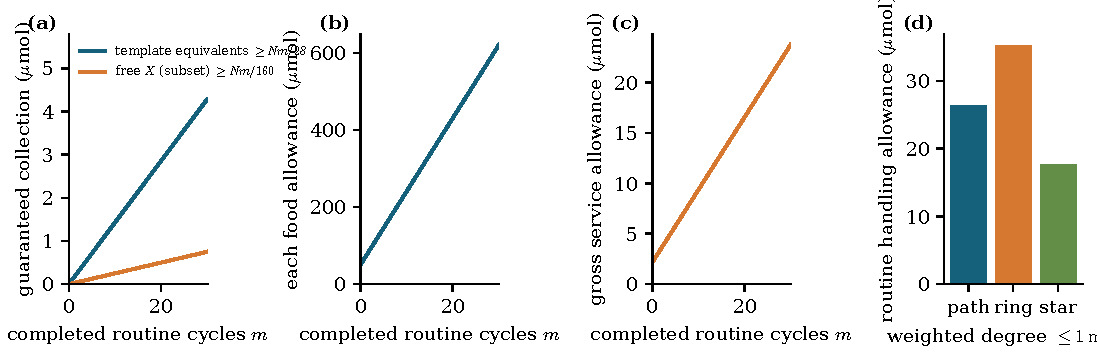
\includegraphics[width=\linewidth]{accounts.pdf}
\caption{Analytic guarantees and allowances for the four-node array. (a) Collection lower bounds after $m$ routine cycles. (b) Each-food allowance and (c) gross-service allowance including conditioning. (d) Per-cycle handling upper bounds at equal maximum weighted degree, so the star uses a smaller per-edge coefficient. None of these lines or bars estimates optimal performance or apparatus energy.}
\label{fig:accounts}
\end{figure}

\section{Scope and the transport boundary}\label{sec:scope}

\subsection{Species-selective exchange breaks the minimum-drift argument}
\begin{proposition}[Exact selective-exchange witness]\label{prop:selective}
Take two nodes with $r=21$, $\delta=1/25$ and states $c_1=(151/160,151/160,1/20,0,0,0)$ and $c_2=(1033/1120,1033/1120,0,0,1/28,0)$, both with $A=B=159/160$ and $Y=1/20$, and exchange only the free template $X$ with coefficient $2$. Then at node $1$, which minimizes $Y$,
\begin{equation}\label{eq:witness}
\frac{\dd}{\dd t}Y(c_1)=(\eps+\delta\eta)\Bigl(\frac{151}{160}\Bigr)^2+\Bigl(\frac52\cdot\frac{151}{160}-1-\delta-\frac{\eps}{10}\Bigr)\frac1{20}-\frac r5\Bigl(\frac1{20}\Bigr)^2-\frac1{10}
=-\frac{227999990907999}{5120000000000000}<0 .
\end{equation}
\end{proposition}
\begin{proof}
The selective transport contributes $2(x_2-x_1)=-1/10$ to $x_1'$ and hence to $Y(c_1)'$; the rest is~\eqref{eq:Ydrift}. The value is exact rational arithmetic.
\end{proof}
The two states have equal weighted stock in different phases; selective transport removes free template from node~1 without bringing the complexed phase that node~2 holds. Thus the species-independence hypothesis has mathematical content: with it, transport is nonnegative at a minimizing node for \emph{every} linear observable simultaneously; without it, the favourable sign fails for the observable that drives recovery. The witness does not prove extinction or rule out a different recovery theorem for selective transport; it delimits the connection rule.

\subsection{Withdrawal, refill and dilution}\label{sec:dilution}
The pulse map~\eqref{eq:pulse} is the endpoint of a withdrawal followed by a volume-restoring refill. Start from volume $V$ and dimensional concentrations $c^-$. Withdraw $(1-q)V$ of well-mixed fluid; the retained amount of species $s$, after the permitted additional loss, is $q\ell_sVc_s^-$. Refill to volume $V$ with a food solution: the resulting concentration is $q\ell_sc_s^-$, exactly the non-food part of~\eqref{eq:pulse}, so dilution by the restored volume is included. The food streams supply amounts $(1-q+e_U)c_0V$ and $(1-q+e_W)c_0V$, that is, refill concentrations $c_0(1+e/(1-q))\in[0.98c_0,1.02c_0]$ over the admitted ranges. The remaining idealization is temporal: reaction, mixing, exchange and collection during the withdrawal and refill are collapsed into an instantaneous map. Validating a finite-duration implementation requires bounding its actual endpoint error and proving that the subsequent return still lands in $\Bstar^N$; because $\Bstar$ is closed and the theorem certifies return \emph{to} it rather than into its interior with a quantified margin, a generic continuity statement is not sufficient.

\subsection{Unequal volumes}\label{sec:volumes}
The theorem is stated for equal volumes, as formalized. With fixed positive volumes $V_i$ and symmetric volumetric exchange rates $q_{ij}$, the operator becomes $(\Dop v)_i=V_i^{-1}\sum_jq_{ij}(v_j-v_i)$. It still satisfies Lemma~\ref{lem:transport}\ref{it:commute} and~\ref{it:min}, so Sections~\ref{sec:transport}--\ref{sec:phase} carry over verbatim, while the summed identity becomes $\sum_iV_i(\Dop v)_i=0$, so the accounts of Section~\ref{sec:repetition} become volume-weighted amounts. We record this as a conventional remark; it is not part of the compiled statement, and a count-level formulation would also have to carry the volume factors in the directional coefficients.

\subsection{What is not modelled and what remains open}\label{sec:open}
The result is an externally operated well-mixed reactor-array model with instantaneous synchronized pulses, restored volumes, maintained activities, bulk nonselective exchange and a schematic effective chemistry. The reverse service reaction has three reactants; an elementary expansion through an intermediate ($U+W\rightleftharpoons H$, $H+P\rightleftharpoons X+F$) would add a species, occupancy, washout and transport, and needs its own inequalities or a quantified approximation over the mission, so the present paper describes the service reaction as an effective maintained mechanism and claims no elementary realization. The declared fuel potential difference $\log(8\cdot10^{10})\,k_BT\approx25.1\,k_BT$, about $62.2\,\mathrm{kJ/mol}$ at $298$ K, is a model parameter. Gross service and handling counts omit food supply, activity maintenance, collection, mixing, pumping and separation.

Four extensions are well posed and open. (1) A finite-duration intervention with a certified endpoint error and a strict return margin. (2) Membranes that retain catalysts while passing foods: Proposition~\ref{prop:selective} shows one obstacle; the full problem also changes washout and needs volume, selectivity and resource balances. (3) A stochastic assembly: inter-node transfer adds count-process jumps, and the finite-molecule reliability theorem of~\citep{finiteharvest2026} for one reactor cannot be imported without a new generator and a uniform repeated-success estimate. (4) An autonomous finite bath whose depletion changes the reaction law continuously rather than through a cutoff. A sharper free-template floor, as Remark~\ref{rem:slack} explains, needs a new uniform inequality rather than a better exponential.

\section{Discussion}\label{sec:discussion}
The theorem makes a precise prediction from component certificates. One local growth inequality below a stock threshold, one phase-sensitive observable, and three properties of common transport certify that any finite conservatively exchanging assembly of these reactors returns after every synchronized intervention and collects a fixed amount of free product at every node, without solving the assembled nonlinear state space and without any dependence on the exchange strength. Material contraction fixes the food corridor; growth at the least-stock node recovers catalytic stock; a backward-evolving weight converts that stock into free product; conservation ties the same history to common supply and synthesis accounts. Uniform floors coexist with architecture-dependent trajectories and handling costs, which is what one wants from a composition theorem: the guarantee is a property of the module and the connection rule, the cost is a property of the architecture.

Two features of the proof deserve emphasis. First, the improvement of the free-template floor from $1/540$ to $1/209$ to $1/160$ came from respecting correlations in the material constraint and from retaining the distinct phase losses in a positive lower comparison system, not from fitting a favourable simulated trajectory; the exact exponential of the same lower system would add only two percent more. Second, the boundary of the connection rule is exact: species-selective exchange defeats the favourable sign at a minimizing node for the very observable that drives recovery. The immediate empirical question is whether a candidate reaction module's measured rates and operating disturbances lie in the certified boxes; the theorem then supplies a checkable sufficient operating criterion for arrays of such modules, without identifying a laboratory realization.

\paragraph{Data and code availability.}
The LaTeX source, the bibliography, the figure data and scripts, the exact replay script and the verification receipts are distributed with this manuscript. \RepositoryNote

\appendix
\section{Formal scope and reproduction}\label{app:formal}
The conventional argument of Sections~\ref{sec:transport}--\ref{sec:repetition} is self-contained. Its central statements are additionally verified in Lean~4 (toolchain \lean{leanprover/lean4:v4.30.0}) against a frozen Mathlib manifest, with warnings treated as errors, in the namespace \lean{C4Assemblies} under \lean{proofs/C4Assemblies/}. The verifier exports the elaborated interface of each requested declaration and lists its axioms; every exported declaration uses only \lean{propext}, \lean{Classical.choice} and \lean{Quot.sound}, and no \lean{sorry}, admitted proposition or native numerical certificate enters. Local kinetics, interventions and regions are imported from the verified development of~\citep{recovery2026} (namespace \lean{ProductiveRecovery}); the cleavage speed is named \lean{d} there, and the phase coordinates are indices $2$--$5$ of a \lean{Fin 6} vector.

\begin{longtable}{>{\raggedright\arraybackslash}p{0.30\linewidth}>{\raggedright\arraybackslash}p{0.64\linewidth}}
\caption{Claims and their formal interfaces.}\label{tab:claims}\\
\toprule Claim & Lean declaration(s) or proof boundary\\\midrule\endfirsthead
\toprule Claim & Lean declaration(s) or proof boundary\\\midrule\endhead
Coupled field equals chemistry plus directed transfers; transfer marks & \lean{literal_assembly_field}, \lean{literal_transfer_drift}, \lean{transferExportMark}, \lean{transferFoodMark}, \lean{transferHandlingMark}\\
Elemental and potential balance of transfers; common thermochemistry at every node & \lean{transfer_element_balance}, \lean{transfer_potential_balance}, \lean{transfer_thermochemistry}, \lean{node_common_thermochemistry}\\
Lemma~\ref{lem:transport} & \lean{diffusion_add}, \lean{diffusion_mul}, \lean{diffusion_const}, \lean{diffusion_at_min}, \lean{diffusion_at_max}, \lean{diffusion_sum_zero}; commutation for $A,B,Y$ and the phase weights: \lean{assembly_A}, \lean{assembly_B}, \lean{assembly_Y}, \lean{phaseWeight_assembly}\\
Lemma~\ref{lem:comparison} & \lean{finite_strict_lower_barrier} (strict form, continuous induction on a closed set), \lean{finite_lower_barrier}, \lean{finite_upper_barrier}, \lean{diffusion_lower_bound}\\
Proposition~\ref{prop:existence} & \lean{assembly_global_nonnegative_solution} (cutoff and positive-part construction, total-material barriers), \lean{assembly_actual_unique}\\
Lemma~\ref{lem:pulse} & \lean{pulse_material}, \lean{pulse_catalyst}, \lean{pulse_nonnegative}, \lean{food_feasible} (isolated development)\\
Lemma~\ref{lem:material} & \lean{material_decay}, \lean{corridor_from_decay}, \lean{assembly_material_bounds}\\
Lemma~\ref{lem:growth} & \lean{weighted_drift}, \lean{strong_guarded_growth} (isolated), \lean{assembly_guarded_growth_at_min}\\
Lemma~\ref{lem:fence}, Proposition~\ref{prop:return} & \lean{assembly_scheduled_recovery}, \lean{assembly_trajectory_return}, \lean{assembly_conditioning_return}, \lean{assembly_routine_return}, \lean{exists_assembly_conditioning}, \lean{exists_assembly_routine}\\
Lemma~\ref{lem:phases} & \lean{sharp_phase_comparison} (common loss $48$), \lean{fine_phase_comparison} (distinct losses $48,43,41,24$ with the $2z$ link)\\
Lemma~\ref{lem:backward}, certificate A & \lean{sharp_backward_phase_local}, \lean{sharp_backward_phase_deriv}, \lean{sharp_phase_minimum_propagation}; floor $1/209$: \lean{sharp_assembly_free_phase_floor}, \lean{sharp_assembly_routine_free_export}\\
Lemma~\ref{lem:backward}, certificate B & \lean{finePhaseWeight}, \lean{finePhaseWeight_assembly}, \lean{fine_backward_phase_local}, \lean{fine_backward_phase_deriv}, \lean{fine_phase_minimum_propagation}; exponential bound \lean{fine_exp_twelve_sevenths}; floor $1/160$: \lean{fine_assembly_free_phase_floor}, \lean{fine_assembly_routine_free_export}\\
Template inventory $\Iv\ge\frac57Y$; $\Iv\le A,B$ & \lean{inventory_lower}, \lean{inventory_le_material}\\
Lemma~\ref{lem:budgets}, Proposition~\ref{prop:segment} & \lean{gross_service_bound}, \lean{assembly_routine_output_supplies}, \lean{assembly_conditioning_supplies}\\
Proposition~\ref{prop:recursion} & \lean{completedSegment}, \lean{Protocol}, \lean{routineHistory}, \lean{arbitrary_assembly_operation}\\
Lemma~\ref{lem:inventory}, Proposition~\ref{prop:synthesis} & \lean{assembly_inventory_balance}, \lean{assembly_pulse_inventory}, \lean{synthesis_telescoping}, \lean{conditioned_mission_synthesis}, \lean{ready_mission_synthesis}, \lean{conditioned_threshold}, \lean{ready_threshold}\\
Theorem~\ref{thm:main}\ref{it:traj}--\ref{it:accounts} as one declaration & \lean{conservative_assembly_operation} (floor $1/540$), \lean{sharp_conservative_assembly_operation} ($1/209$), \lean{fine_conservative_assembly_operation} ($1/160$)\\
Closed four-node instances on~\eqref{eq:example} & \lean{pathParameters}, \lean{ringParameters}, \lean{heterogeneousReady}, \lean{heterogeneous_ready}, \lean{fixedPulse}, \lean{nonzero_distinct_topologies}, \lean{fine_path_operation}, \lean{fine_ring_operation} (and the \lean{sharp_} and unprefixed versions)\\
Remark~\ref{rem:cutoff}, handling~\eqref{eq:handling}, ceiling~\eqref{eq:ceiling} on one segment & \lean{source_prefix_allowances}, \lean{source_prefix_cutoff_agreement}, \lean{common_mission_prefix_allowance}, \lean{source_transport_allowance}, \lean{assembly_food_ceiling}\\
Mission sizing, endpoint rates, degree and edge scaling, multi-segment ceiling, dimensional conversions, dilution derivation, unequal volumes & Conventional (Sections~\ref{sec:consequences}, \ref{sec:units}, \ref{sec:scope})\\
Proposition~\ref{prop:selective} & Exact rational substitution (replayed by the check script), not a Lean declaration\\
Pilot trajectories, Table~\ref{tab:pilot}, Figures~\ref{fig:recovery}--\ref{fig:accounts} & Sampled numerical integration, not kernel-checked enclosures\\
\bottomrule
\end{longtable}

\paragraph{Root declaration.}
The declaration \lean{fine_conservative_assembly_operation} takes a \lean{Parameters} structure (exchange matrix with nonnegativity, symmetry and zero diagonal, node parameters with the four interval bounds), an initial intervention vector, a \lean{Protocol} (a function of the cycle index, the list of completed segments and the current assembly), an assembly and a proof that it is admitted; it produces the conditioning trajectory $C$, the states $s_n$, the routine trajectories $X_n$ and the histories $H_n$ with: $C(0)=\Pulse_{p^0}c$; nonnegativity and the derivative identity for all $t\ge0$; $s_0=C(12)$, $H_0=[]$; every $s_n$ ready; for every $n$, $X_n(0)=\Pulse_{\Pi(n,H_n,s_n)}s_n$, $X_n(4)=s_{n+1}$, $H_{n+1}$ is $H_n$ with the clipped segment prepended, nonnegativity and the derivative identity, readiness at times $3$ and $4$, and $x_i\ge1/160$ on $[3,4]$ at every node; and for every $m$ the five summed inequalities~\eqref{eq:accounts}. The declarations \lean{sharp_conservative_assembly_operation} and \lean{conservative_assembly_operation} have the same statement with $1/209$ and $1/540$. The two synthesis declarations take the same trajectory data as hypotheses and conclude the net-synthesis inequalities of Proposition~\ref{prop:synthesis}.

\paragraph{Receipts.}
Verification receipts are JSON files written by the repository's verifier: \lean{Examples.verify.json} (root with floor $1/540$, path and ring instances, conditioned synthesis), \lean{Publication.verify.json} (floor $1/209$, instances, ready-start synthesis, free export) and \lean{PublicationFine.verify.json} (floor $1/160$, instances, free export). Each records the toolchain, the manifest hash, the source hash of the target, the hashes of all dependency sources and artifacts, the exported interfaces and the compiler streams, which are empty.

\paragraph{Reproduction.}
From the repository root, with the repository's Python interpreter, the strict verification of the strengthened root is
{\small\begin{verbatim}
.venv/Scripts/python.exe scripts/verify_proof.py
    proofs/C4Assemblies/PublicationFine.lean
    --declaration C4Assemblies.fine_conservative_assembly_operation
    --declaration C4Assemblies.fine_path_operation
    --declaration C4Assemblies.fine_ring_operation
    --declaration C4Assemblies.fine_assembly_routine_free_export
    --output problem_workspaces/RAF_C4_composition_on_defined_assemblies/
             PublicationFine.verify.json
\end{verbatim}}
(one command on one line; the argument lines are wrapped here and the output path is split only for display), and likewise for \lean{Publication.lean} with the \lean{sharp_} declarations and \lean{ready_mission_synthesis}, and for \lean{Examples.lean} with the unprefixed declarations. The pilot is \lean{figures/diagnostic.py}; \lean{make_figures.py} draws Figures~\ref{fig:recovery} and~\ref{fig:accounts} from the saved traces \lean{figures/trajectory_data.npz} and \lean{figures/figure_data.json}; \lean{check_paper.py} re-derives every identity, inequality, certificate and printed number of this paper in exact arithmetic (one hundred checks). Compile with \lean{pdflatex}, \lean{bibtex}, and two further \lean{pdflatex} passes. No numerical integration is needed to verify the theorem.

\small
\bibliographystyle{plainnat}
\bibliography{refs}

\end{document}
